\documentclass[11pt,a4paper]{article}
\usepackage[T1]{fontenc}
\usepackage{lmodern}
\usepackage{amsmath,amssymb,graphicx,booktabs,array,tabularx}
\usepackage[margin=1in]{geometry}
\usepackage{natbib}
\usepackage[hidelinks]{hyperref}
\usepackage{microtype}
\usepackage{caption}
\usepackage{placeins}
\hypersetup{pdftitle={Supplementary Material: Repeated-call evaluation of sensor-mapping faults and batch context in LLM-based industrial fault diagnosis},pdfauthor={Song Ouyang},pdfkeywords={fault diagnosis, large language models, sensor mapping, repeatability}}
\captionsetup{font=small,labelfont=bf}
\setlength{\textfloatsep}{16pt plus 3pt minus 3pt}
\setlength{\intextsep}{14pt plus 3pt minus 3pt}
\clubpenalty=10000
\widowpenalty=10000
\setlength{\emergencystretch}{2em}
\renewcommand{\topfraction}{0.85}
\renewcommand{\textfraction}{0.10}
\renewcommand{\floatpagefraction}{0.75}
\setcounter{topnumber}{3}
\setcounter{totalnumber}{4}
\newcommand{\NA}{\textemdash}
\usepackage{xcolor}\newcommand{\todo}[1]{\textcolor{red}{[TODO: #1]}}

\title{Supplementary Material for ``Repeated-call evaluation of sensor-mapping faults and batch context in LLM-based industrial fault diagnosis''}
\author{Song Ouyang\\[2pt]\small Independent Researcher, Chengdu, Sichuan, China}
\date{}

\graphicspath{{./}}
\begin{document}
\maketitle
\noindent\textbf{Contents.} Sections 1--7 reproduce the report of the preliminary stages (a 130-source paired study of five LLM services, a representation and context follow-up, a DeepSeek/Qwen API addition and the source-disjoint follow-up), with extended methods, all repeated outcomes and protocol amendments; its original numbering is retained. Appendix~A lists audit controls. Appendix~B documents two non-controlled Claude collections that are excluded from every analysis in the main paper. Appendices~C and~D give the first hydraulic run and the post hoc repetition and timing audit, and Appendix~E the ABBA/BAAB replication. Appendix~F reports the full inferential statistics, Appendix~G the completion of the hydraulic study, and Appendix~H the tuned supervised baselines.

\section*{Summary of the preliminary report}
Correct fault labels do not establish that a large language model (LLM) uses sensor descriptions correctly. We examine this distinction in an exploratory paired study of 60 held-out C-MAPSS engines and 70 held-out Tennessee Eastman Process (TEP) runs. Three GPT services receive clean inputs and a TEP descriptor rotation that preserves numerical strings and positions. Supervised references use the same rounded features. Primary TEP accuracy losses are 28.6 percentage points for GPT-5.5 (conditional 95\% interval [11.4, 45.7]) and 77.1 for GPT-5.6 Sol ([67.1, 87.1]); GPT-6 Astra has unchanged labels. A separate 84-request follow-up tests field reordering, descriptor removal, noncyclic corruption and context. For seven matched cases, repeat-1 correct counts change from 7/7 to 2/7 for Sol and from 7/7 to 6/7 for Astra when the surrounding 63 records are removed. An additional DeepSeek/Qwen study yields 15/18 valid responses: Qwen's primary corruption loss is 22.9 percentage points, whereas DeepSeek's primary corrupted response is invalid. A further 84-request follow-up adds 172 disjoint sources, multiple mappings, crossed context controls and FD002 transfer. Across all stages, 209/213 responses are valid on 302 source units. Primary FD002 accuracy is 60.0\% for Sol and 71.7\% for Astra. Uncertainty is conditional on the observed grouped responses. Tool-enabled conversational records are reported separately and excluded from the controlled comparisons. The findings distinguish mapping sensitivity from classification accuracy and motivate reporting context effects and response availability alongside scores; they establish neither internal reasoning mechanisms nor industrial generalizability.

\noindent\textbf{Keywords:} industrial monitoring; large language models; sensor mapping; fault classification; context sensitivity; reproducibility

\section{Introduction}
Industrial monitoring systems associate each measurement with a sensor identity, physical quantity and unit before interpreting an equipment state. Statistical feature extraction and supervised learning are established approaches to this task \citep{lei2020applications,zhao2019deep}. General-purpose LLMs introduce a text interface: numerical observations and engineering descriptions are serialized together, and the model returns a diagnostic category without fitting task-specific parameters. This makes the correctness of the serialization itself part of the evaluation problem.

Consider a schema-conversion error that assigns a temperature descriptor to a pressure value while preserving the original number. A lower classification score would reveal sensitivity to that error. An unchanged score is harder to interpret: the model may ignore the descriptor, rely on a familiar numerical position, or recognize and compensate for the conversion fault. Accuracy alone cannot distinguish these explanations. The same ambiguity arises at the request level. When many observations share a context, an individual prediction may depend on other observations or their order, even when the task asks for independent classification.

Existing research already studies sensor-to-text representations and task-specific adaptation \citep{qaid2026explainable,zheng2024empirical}. Our focus is the narrower evaluation question of whether successful label prediction under a text interface also demonstrates dependence on a valid mapping, and how response completeness and repeated sessions constrain that inference. We separate three observable properties: classification performance, prediction sensitivity to a specified mapping fault, and repeatability of the service response. Source-unit separation and shared numerical inputs control these comparisons.

The original experiment addresses two questions:
\begin{enumerate}
\item With numerical strings and positions fixed, how does an incorrect sensor-descriptor mapping affect both accuracy and individual predictions?
\item For the same grouped input, how do complete-response coverage and repeated-session disagreement qualify the interpretation of those scores?
\end{enumerate}
Supervised comparisons on the same observations characterize task difficulty under the respective training interfaces.

The study makes three connected contributions. First, it pairs a fully specified descriptor fault with unchanged numerical observations and reports both accuracy differences and case-level decision changes. Second, separately frozen follow-ups test whether mapping invariance persists under representation and context changes and extend the comparison to two additional provider APIs. Third, complete request records and fail-closed scoring preserve the distinction between usable output and classification performance. These contributions concern evaluation practice rather than a new diagnostic architecture. The first two follow-ups reuse the original observations. A third, prospectively specified follow-up adds disjoint source runs, multiple mapping realizations, a crossed context design and an FD002 transfer panel. It tests the reach of the earlier observations, while remaining exploratory and conducted by the same study workflow.

\section{Related work and study position}
Machine-health monitoring research encompasses feature-based learning, deep models and evaluation across operating conditions \citep{lei2020applications,zhao2019deep}. Unit-based evaluation addresses the dependence introduced by splitting related signal segments across training and testing \citep{vieira2026realistic}. We adopt this established principle for engines and simulation runs. It protects the supervised comparison from source overlap but does not remove dependence among predictions generated in a shared LLM context.

FD-LLM encodes machine signals through frequency-domain or statistical representations and uses instruction fine-tuning for diagnosis \citep{qaid2024fdllm}; related journal work studies explainable diagnosis \citep{qaid2026explainable}. Zheng et al.\ investigate language-model fine-tuning for complex-system diagnosis \citep{zheng2024empirical}. These studies motivate treating the text interface as an experimental factor. Here, exact measurements are retained while complete physical descriptors are reassigned, and the resulting decision changes are compared with repeated fresh requests. We do not infer priority from differences in terminology or directly compare published scores across different tasks.

Kiangala and Wang combine repeated structured diagnostic outputs, training-reference retrieval and an independent verifier for selective diagnosis \citep{kiangala2026verification}. Their separation of raw labels, agreement and accepted-case coverage is relevant to our reporting distinction. Our experiment instead targets controlled changes in the supplied measurement mapping and co-presented observations. It measures label changes under those interventions; it does not evaluate rationale grounding or an acceptance-and-escalation classifier.

FailureSensorIQ probes relationships between industrial sensors and failure modes through knowledge questions \citep{constantinides2025failuresensoriq}. SensorBench evaluates coding-based sensor processing \citep{sensorbench2025}, and industrial chain-of-thought distillation studies task-specific training \citep{lin2025finetuned}. These tasks address capabilities beyond direct label prediction from a numerical snapshot. Their task definitions provide context for the scope of our direct classification interface. Table~\ref{tab:position} states the operational distinction between the closest research directions and this study.

A recent automotive preprint converts hardware-in-the-loop sensor windows into statistical, relational and contextual descriptions and adapts open language models to fault-location prediction \citep{abboush2026sensor}. It strengthens the motivation for examining sensor-to-text interfaces, but its task-specific adaptation and fault-injection setting differ from the fixed, general-purpose services assessed here. We do not compare scores across those different tasks or treat that preprint as independent validation of our findings.

\begin{table}[htbp]
\centering\small
\caption{Study position relative to closely related work. The distinctions specify evaluation scope, not priority claims or superiority.}
\label{tab:position}
\begin{tabularx}{\linewidth}{@{}>{\raggedright\arraybackslash}p{0.31\linewidth}>{\raggedright\arraybackslash}X@{}}
\toprule
Research direction & Relationship to the present question \\
\midrule
Signal-to-language diagnosis \citep{qaid2026explainable} & Establishes representation and task-adaptation approaches. Here, fixed general-purpose services receive numerical text without task-specific training. \\
Complex-system fine-tuning \citep{zheng2024empirical} & Studies task adaptation through a text interface. Here, a fully specified incorrect mapping is paired on identical observations and examined through both score changes and decision flips. \\
Repeated outputs and verification \citep{kiangala2026verification} & Separates agreement, verification and selective coverage. Here, controlled descriptor and context changes are the exposure of interest. \\
Sensor--failure knowledge \citep{constantinides2025failuresensoriq} & Tests industrial knowledge through questions. Here, the prediction concerns a specific measured state whose text mapping may be incorrect. \\
Coding-based processing \citep{sensorbench2025} & Allows code-mediated signal processing. Here, the interface returns labels with tools disabled and retains invalid responses in coverage reporting. \\
\bottomrule
\end{tabularx}
\end{table}

\section{Data preparation and experimental design}
\subsection{Study stages and scope of inference}
The original experiment is an exploratory paired comparison. Its completed results motivated separately planned representation/context and additional-provider follow-ups, both reusing the original 130 source units. A fourth stage introduces 172 previously unused sources: 112 TEP simulation runs and 60 FD002 engines. Each follow-up retains its own protocol and prediction freeze. Table~\ref{tab:stages} distinguishes requests, valid outputs and repeated classifications. Across stages, the source count is 302; repeated calls and earlier observations from the same runs do not add independent sources. The source-disjoint follow-up was planned after seeing earlier results and is not an original preregistration or an independent-team replication. Two separate Claude collections---an earlier historical submission and a later tool-enabled conversational exploration---are retained in Appendix~\ref{app:claude_reported}. Neither has a verified inference-provenance chain, and both are excluded from all controlled request and source totals.

\begin{table}[htbp]
\centering
\small
\caption{Evidence stages. Valid labels count repeated classifications, not independent assets. The first three stages reuse 130 sources; the last adds 112 TEP runs and 60 FD002 engines. Both historical and tool-enabled conversational Claude records are excluded.}
\label{tab:stages}
\begin{tabular}{@{}lrrr@{}}
\toprule
Stage & Requests & Valid & Labels valid/planned \\
\midrule
Original paired study & 27 & 26 & 1,740/1,800 \\
Representation/context follow-up & 84 & 84 & 2,604/2,604 \\
Additional-provider API study & 18 & 15 & 990/1,200 \\
Source-disjoint follow-up & 84 & 84 & 4,854/4,854 \\
Total (302 unique sources) & 213 & 209 & 10,188/10,458 \\
\bottomrule
\end{tabular}
\end{table}


\subsection{Evaluation units and selection}
Figure~\ref{fig:workflow} summarizes the original study workflow and paired intervention; Table~\ref{tab:data} gives the evaluation units. The source datasets are public simulations. Training and testing roles are determined before querying any LLM. Labels, group identities, raw-file hashes and source coordinates are stored separately from the inference payload.

\begin{figure}[htbp]
\centering
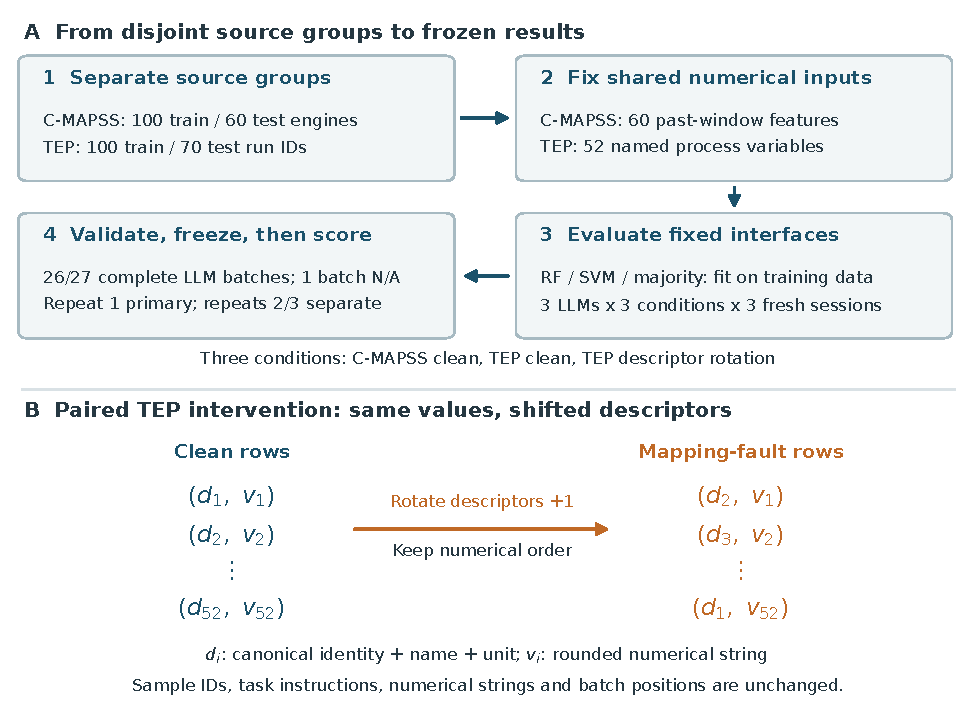
\includegraphics[width=\linewidth]{figures/revision_v3/evaluation_workflow.pdf}
\caption{Original-study evaluation workflow and the symbolic TEP descriptor rotation. Source units are disjoint across training and testing; LLM outputs share a grouped context. Supervised methods fit labeled training data, while LLMs receive task definitions and sensor descriptions. The intervention shifts complete descriptors by one position while retaining the numerical sequence; it does not alter C-MAPSS inputs.}
\label{fig:workflow}
\end{figure}

\begin{table}[htbp]
\centering
\small
\caption{Evaluation units and representations. Test counts refer to unique engines or run IDs, not repeated LLM outputs. TEP training contains seven scenarios per selected run ID.}
\label{tab:data}
\begin{tabular}{@{}lrrrr@{}}
\toprule
Task & Features & Train records & Train groups & Test groups \\
\midrule
C-MAPSS & 60 & 500 & 100 & 60 \\
TEP & 52 & 2100 & 100 & 70 \\
\bottomrule
\end{tabular}
\end{table}


For C-MAPSS, we use the official FD001 training trajectories and official test trajectories with the supplied test remaining-useful-life (RUL) targets \citep{saxena2008damage,saxena2008dataset}. An engine identifier is interpreted jointly with its source split: identical integer identifiers in the two files do not identify the same engine. The test observation is the final available cycle of each selected engine. Its supplied RUL defines three operational categories: Healthy for $\mathrm{RUL}>80$, Degrading for $30<\mathrm{RUL}\leq80$, and Critical for $\mathrm{RUL}\leq30$. These thresholds define a retrospective health-staging proxy; they are not observed fault mechanisms or validated maintenance thresholds.

The available test labels comprise 55 Healthy, 20 Degrading, and 25 Critical engines. A fixed random seed selects 20 from each class. We retain one observation per test engine and randomize the input order independently of class. Training windows are extracted only from official training engines. The label may use the complete training trajectory to calculate historical RUL, while each feature vector uses only measurements available by its observation time. No true RUL, engine identifier, absolute cycle number, or future measurement enters the LLM input or supervised feature vector.

For TEP, we use the raw fault-free and faulty \emph{Training} files of the expanded simulation dataset \citep{downs1993plant,rieth2017additional}. We construct a new run-level split within these files; the word ``test'' below refers to our held-out runs, not the publisher's separate Testing files. The source documentation states that training faults are introduced after one hour and measurements are sampled every three minutes. Selected observations occur at sample indices 200--500, well after fault injection. They represent established post-fault operation, without assuming that every affected process has reached a steady state. Consequently, this task does not evaluate early detection or time to alarm.

The seven conditions are Normal and faults 1, 2, 4, 6, 7, and 13. These fault types form a convenience subset fixed before inference, rather than a representative sample of all TEP fault mechanisms. Training uses 100 simulation-run identifiers. The 70 test observations use 70 additional, globally distinct run identifiers, with ten observations per condition. A run identifier is excluded from training across \emph{all} fault conditions, preventing condition-specific splitting from reusing the same simulation seed group. A single selected observation is retained from each test run. This balanced subset supports a manageable stress test; its class prevalence does not represent a production process.

\subsection{Common numerical representation}
For C-MAPSS, 15 nonconstant sensor channels are selected using training-data variation only: sensors 2, 3, 4, 6, 7, 8, 9, 11, 12, 13, 14, 15, 17, 20, and 21. Each observation summarizes exactly 30 available cycles. For a channel $x_1,\ldots,x_{30}$, the representation contains its mean, population standard deviation, least-squares slope against the within-window index, and last value. The result is a 60-dimensional vector. Window lengths, feature precision and channel descriptors are checked against the data manifest.

TEP observations contain all 41 measured variables and 11 manipulated variables. Extraction addresses the canonical source column names explicitly rather than assigning descriptors by dataframe position. The source fields \texttt{faultNumber}, \texttt{simulationRun}, and \texttt{sample} are retained as provenance or labels and excluded from the feature vector. Each of the 52 numerical entries receives its documented descriptor and unit in the clean text representation; variable identities follow the TEP specification, with units checked against the original operating tables \citep{chen2014cognitive,ricker1995optimal}.

Both tasks round values before either classifier family receives them. The same rounded arrays train and evaluate RF/SVM and generate LLM sensor text. This eliminates a hidden precision advantage for the numerical baselines. The models still differ in information and training: LLMs receive channel names, units, task definitions, and their pretrained knowledge, while supervised models fit labeled training examples. The comparison is between these practical task interfaces, not between equally trained architectures.

The LLM instruction defines the permitted labels and the task. TEP fault identifiers are accompanied by fixed mechanism descriptions so that the label vocabulary is interpretable. There are no labeled in-context examples or train-set-derived normal-value summaries. We describe this as zero-shot task prompting, while recognizing that familiar benchmark information may already occur in pretraining.

\subsection{Paired descriptor-mapping intervention}
The TEP stress test keeps every test observation, anonymous ID, numerical string, task definition, and within-batch position fixed. Only the mapping of the 52 sensor descriptors is changed. Let $d_i$ include the canonical sensor identity, descriptive name, and unit, and let $v_i$ be the corresponding numerical string. Clean rows contain $(d_i,v_i)$. The corrupted condition contains
\begin{equation}
  (d_{1+(i\bmod 52)},v_i),\qquad i=1,\ldots,52.
\end{equation}
Thus the descriptor sequence is cyclically shifted by one place, with the final row receiving $d_1$. The numerical sequence is unchanged. Preparation checks that exactly 52 fields are transformed and that the paired IDs and order agree. The corrupted condition is named \texttt{misnamed} in the archived files and plots.

This synthetic, deliberately severe schema fault changes physical interpretation and may create conspicuous range inconsistencies, because units travel with the descriptors. The intervention measures sensitivity to this specific reassignment. It combines changes to sensor identities, names and units, so their individual effects and the model's internal diagnostic mechanism remain unresolved.

\subsection{Inference protocol and response validation}
We request \texttt{gpt-5.5}, \texttt{gpt-5.6-sol}, and \texttt{gpt-6-astra}, each with the \texttt{medium} reasoning setting through a ChatGPT-authenticated Codex CLI over HTTPS. Each model receives C-MAPSS clean, TEP clean, and TEP corrupted inputs in three fresh sessions: $3\times3\times3=27$ sessions. The 60 or 70 observations for a condition share one context. The 1,800 requested classifications correspond to 130 unique simulated evaluation units, not 1,800 independent samples. The Results section reports actual response completeness separately from classification performance.

The sample order is a fixed random permutation, reused across paired conditions and repeats. A deterministic per-model shuffle of the nine session jobs reduces a fixed ordering of conditions over time. Each inference process starts in an empty temporary directory; user configuration, project instructions, skills, plugins, web search, and tools are disabled. The payload contains anonymous IDs and prompts, while the execution process does not open answer files. A shared instruction forbids deriving labels from IDs, neighboring observations, or assumed class balance. These instructions reduce obvious shortcuts but cannot remove dependence created by a shared context.

Responses must contain one JSON array with exactly one \texttt{id}/\texttt{predicted} object per input, in the original order. Labels must match the permitted spelling and case exactly. The validator rejects missing or duplicate IDs, extra fields, invalid labels, tool events, and incomplete execution logs. It does not extract labels by substring or revise predictions after seeing their accuracy. At most two attempts are permitted for transport failure; a semantic output failure is recorded and fails closed rather than triggering score-guided repair.

The original frozen protocol specified fail-closed validation, but the initial scorer required every batch to succeed. After an incomplete response was observed, and before computing LLM classification metrics or linking predictions to answer keys, we recorded a timestamped failure-reporting amendment. It assigns N/A to the entire invalid batch and reports validity separately, without scoring partial labels or replacing a failed primary session. This missing-data reporting rule was amended before scoring; it was not part of the original protocol. Remaining never-attempted jobs continued, while the failed response was retained without a semantic retry.

Before scoring, the workflow freezes the prediction files and all request, response, metadata, and event logs with SHA-256 hashes. The scorer verifies the frozen files before loading answer labels. The requested aliases, reasoning effort, CLI version, timestamps, token usage, and observed tool events are recorded. The CLI does not expose an immutable server-resolved model snapshot, temperature control, or every provider-side instruction. These limitations remain part of the experimental record; an explicitly requested model alias is not proof of fixed model weights.

\subsection{Matched supervised baselines}
The Random Forest (RF) uses 300 trees and a fixed random seed. The support vector machine (SVM) applies training-fitted standardization followed by an RBF kernel with $C=1$ and \texttt{gamma=scale}. Hyperparameters are fixed before test evaluation. The training-majority classifier predicts a single label chosen from training frequencies, with a documented deterministic tie rule. Uniform random guessing and prior-proportional random guessing are reported as expected accuracies, not realized model runs.

These are transparent reference baselines, not an exhaustive optimized supervised benchmark. All supervised models use the same selected test observations and rounded feature arrays as the clean LLM condition. No random-row cross-validation score is substituted for held-out performance. Training-group overlap with test groups must be zero before fitting. The corrupted TEP condition is used to audit the text mapping; unchanged numerical RF/SVM predictions would not be a meaningful test of that text conversion.

\subsection{Exploratory representation and context probes}
After inspecting the original results, we designed a separate exploratory TEP extension for GPT-5.6 Sol and GPT-6 Astra, selected because their observed mapping responses contrasted. The extension reuses the same 70 held-out runs; it adds no independent test sources and is not a confirmatory replication. Its protocol, transformation code, request order and label-free payloads were frozen before the new calls. All new outcomes were frozen before this extension was scored. Historical primary responses were neither replaced nor pooled with these calls.

Six full-batch conditions each receive three fresh sessions per model: the unchanged clean input; the original cyclic descriptor fault; a seeded joint reordering of correct descriptor--value pairs; anonymous positional field labels replacing sensor identities, names and units; one seeded noncyclic descriptor derangement with no fixed points; and a seeded reordering of the clean observations. Joint field reordering preserves all physical pairings, whereas the random mapping fault preserves all numerical strings in their canonical positions. Anonymous inputs retain numerical order and the task-level fault definitions; only sensor-field descriptors and the corresponding row-description sentence change. Each transformation is fixed across samples and repeats. Thus this extension tests particular alternatives to the original rotation, not a distribution of all possible schema faults.

For a bounded context probe, seven observations are selected by the smallest SHA-256 values of a fixed salt concatenated with the anonymous IDs, without using labels or previous predictions. Their original relative order is retained. For each model and repeat, these records are classified together in one seven-record request and in seven independent single-record requests. Their predictions in the fresh 70-record clean batch provide the large-context comparison. This design holds each focal record fixed but changes its surrounding context and position; it does not isolate every aspect of context length. The subset is not class-stratified and is too small for population-level accuracy claims.

The schedule contains 84 requests and 2,604 requested classifications over the original 70 sources. Model aliases and reasoning effort follow the original interface, while every request has a new session. One CLI invocation is permitted per scheduled job; invalid outputs remain unavailable for the entire request, without repair or replacement. Full-batch contrasts and the seven-case context contrasts align by ID, with available-pair denominators reported explicitly. Repeat 1 is the descriptive reference, and repeats 2 and 3 are reported separately. Conditional paired intervals use 10,000 source-unit resamples with seed 20260927; they do not incorporate shared-context dependence or variation over transformations.


\subsection{Exploratory cross-provider API addition}
After the original results and representation/context follow-up, we evaluate two additional service aliases, \texttt{deepseek-v4-pro} and \texttt{qwen3.8-max}, through their provider APIs. This addition repeats the original three task/condition groups and three fresh requests per group, for 18 requests. The original observations, full batch text, order, labels and instruction wording are unchanged. The API system role replaces the original CLI developer-instruction role; no tools are supplied. Repeat 1 remains the primary descriptive comparison, designated in the addition's plan before its requests. No representation/context follow-up conditions are added for these services.

The addition uses a separately versioned, budget-corrected plan. An earlier configuration used a 16,384-token setting whose scope differed between providers; four completed batches were invalid and two active requests were stopped, leaving twelve unattempted jobs. Those records are retained, were not classification-scored, and are excluded from the revised addition. All 18 revised requests were newly scheduled, rather than selectively replacing failures. Both revised payloads cap combined reasoning and final output at 65,536 tokens. DeepSeek uses its high reasoning setting; Qwen additionally caps thinking at 16,384 tokens. These provider-defined controls do not equalize compute or decoding behavior. The correction followed observed execution failures and is not an original-study protocol choice.

Requests follow fixed shuffled submission orders with at most two concurrent sessions per provider and no automatic retries or semantic repair. Complete raw streams, submitted payloads, provider-returned aliases, finish reasons, usage and derived outputs are retained. A manifest freezes every terminal outcome before scoring. The same whole-response validation and paired source-unit analysis apply; an invalid primary is never replaced by a later repeat. The first three stages in Table~\ref{tab:stages} reuse the original 130 source units; the separately described fourth stage adds new sources. None establishes an immutable model-weight snapshot.



\subsection{Source-disjoint follow-up and crossed controls}
After inspecting the first three stages, we froze an additional protocol before its inference. GPT-5.6 Sol and GPT-6 Astra were selected because their earlier responses differed; this selection does not support a population-wide service ranking. The fixed seed is 20260928. Fourteen conditions, two services and three fresh sessions per condition give 84 requests and 4,854 requested labels. The schedule interleaves conditions, including contemporaneous clean controls, with four concurrent requests overall. Each job permits one invocation, no semantic retry or manual repair, and a 900-second timeout. The tool-disabled CLI, medium reasoning setting and whole-batch validation are retained. Every terminal response is frozen before scoring; repeat 1 is primary.

The TEP panel contains 70 new main runs, ten per class, plus two disjoint 21-run background panels A and B, each with three runs per class. Globally, run IDs are excluded across fault scenarios if used in the original training/test split or the historical 50-, 100- or 200-per-class evenly spaced selections. This conservative exclusion removes 365 of the 500 available IDs; 112 of the remaining 135 are selected without inspecting predictions. The preparation audit additionally matches the 1,400 legacy derived rows to raw source coordinates and numerical values. Thus, the main and background panels neither overlap each other nor reuse those prior sources.

The main panel retains one late snapshot per run at a seeded sample index from 200--500. A stratified subset of 21 focal observations covers all seven classes with three observations each. Five context conditions present these identical focal observations alone, before A, after A, before B, or after B. The A/B comparison holds focal position and total size 42 fixed; the front/back comparison holds background identity fixed. The focal-only panel has size 21. Its comparison with size 42 or with the focal subset extracted from the 70-case clean response changes composition as well as size, and cannot isolate a pure size effect. No class quotas or reference labels are supplied to the inference service.

Seven mapping conditions use the identical 70 late observations: clean descriptors, the original one-position rotation, three fixed random derangements of all 52 descriptors, a local swap of reactor-level and separator-level descriptors (both percentages), and a seeded reordering that preserves each correct descriptor--value pair. The five incorrect mappings retain numerical strings and their positions. Correct-pair reordering changes their positions but preserves physical correspondence. The fixed permutations and complete inputs are included in the protocol artifacts; each is reported separately.

Two additional conditions challenge the original task setting. Earlier TEP observations use sample 40 from the same 70 runs, approximately 60 minutes after fault injection, paired with the late snapshots by run. These add observations, not sources, and do not measure early-alarm delay. The FD002 panel selects 60 previously unused test engines, 20 per RUL category, from the official six-operating-condition, one-fault-mode subset. Six of its 259 engines have fewer than 30 available cycles and are excluded; the eligible category counts are 123 Healthy, 69 Degrading and 61 Critical. The final 30 available cycles use the original FD001-selected channels, rounding and 60-feature summary without target-domain adaptation. Operating-setting columns remain excluded as in FD001, so regime variation may affect these summaries. RF and SVM are fit only on the original training features and evaluated once on new late TEP, earlier TEP and FD002 observations. This is a fixed-representation transfer stress test, not a tuned FD002 benchmark.

The stage adds 172 source units and 242 observations, including the 70 same-run earlier snapshots. Its precision rationale is fixed before inference: independent-binomial worst-case 95\% half-widths are approximately 11.4 pp for 70 cases, 12.3 pp for 60 and 20 pp for 21 focal cases. These are feasibility benchmarks, potentially optimistic under grouped generation, not a significance-based power calculation. All repeated outcomes, paired flips and conditional paired bootstrap intervals (10,000 source-pair resamples, seed 20260928) are retained; no permutation or comparison is selected by its score.

\section{Metrics and uncertainty}
\subsection{Target quantities and missing responses}
The primary reported measures are accuracy and macro F1. For $K$ classes, macro F1 is $K^{-1}\sum_{k=1}^K F_{1,k}$, including absent predicted classes with a zero score where appropriate. For C-MAPSS, Critical miss rate is the fraction of true Critical observations assigned another label. For TEP, fault miss rate is the fraction of true fault observations assigned Normal; Normal false-alarm rate is also reported. A correctly recognized Normal class does not imply that faults are detected reliably.

For a valid clean/corrupted pair with $n$ shared observations, let $y_i$ be the reference label and $\hat y_i^{c}$ and $\hat y_i^{m}$ the clean and corrupted predictions. We report
\begin{align}
\Delta_{\mathrm{acc}} &= \frac{1}{n}\sum_{i=1}^{n}\left[\mathbf{1}(\hat y_i^{c}=y_i)-\mathbf{1}(\hat y_i^{m}=y_i)\right],\\
F_{\mathrm{flip}} &= \frac{1}{n}\sum_{i=1}^{n}\mathbf{1}(\hat y_i^{c}\neq\hat y_i^{m}).
\end{align}
Here $\mathbf{1}(\cdot)$ is the indicator function. Positive $100\Delta_{\mathrm{acc}}$ denotes an accuracy loss in percentage points under corruption. $F_{\mathrm{flip}}$ measures changed decisions regardless of correctness. Request-level availability is the number of valid whole responses divided by scheduled requests; label coverage uses the corresponding valid and requested classification counts. An invalid response has no classification score. Thus, conditional accuracy is not an estimate of end-to-end success when unavailable outputs also incur an operational cost.

\subsection{Descriptive accounting for usable correct outputs}
During manuscript revision, after inspecting the frozen scores, we added a descriptive accounting measure for the original and revised API schedules. For one service and task/condition, let $P$ be the number of scheduled classification slots across three repeats, $V$ the number supplied by valid whole responses, and $C$ the number of correct labels within those valid responses. We report
\begin{equation}
Y=\frac{C}{P}=\frac{V}{P}\,A_{\mathrm{valid}},\qquad A_{\mathrm{valid}}=\frac{C}{V}\quad(V>0).
\end{equation}
Here $Y$ is the observed fraction of scheduled slots receiving a usable correct label. An invalid batch contributes its scheduled slots to $P$ but nothing to $V$ or $C$; its classification accuracy remains undefined. If every batch fails, $Y=0$ and $A_{\mathrm{valid}}$ is N/A. This accounting does not score rejected partial outputs, infer what a failed response would have predicted, or replace the designated primary repeat. Because the same observations recur, the counts describe delivered classifications rather than independent sample size; no confidence interval or significance test is added for $Y$. The measure depends on the whole-batch contract and is not a calibrated cost or safety metric.

\subsection{Repeated sessions and conditional uncertainty}

Repeat 1 is designated before inference as the primary descriptive comparison. Accuracy receives a 95\% Wilson interval. Macro-F1 intervals and clean-minus-corrupted paired differences use 10,000 group bootstrap resamples with seed 20260926. Every test group contributes one observation, and paired resampling retains both predictions for that observation. Repeats 2 and 3 are shown separately, together with aggregate score ranges and prediction disagreement; their labels are not pooled as new independent observations. Classification summaries are conditional on a complete valid response. Any unavailable comparison is explicitly recorded, and repeated-session summaries state how many valid sessions contribute.

For any contrast summarized over repeated sessions, the contributing set is the intersection of repeats with complete valid outputs under both conditions. Means from different repeat sets are not treated as paired effects. Missing results are retained as N/A, not assigned zero accuracy or replaced by another repeat. When a sample SD is reported, its denominator is $n-1$ and $n$ is the number of available sessions; a single available session has no estimable SD. These summaries describe the observed sessions rather than estimating a stable distribution of provider behavior.

The intervals are conditional summaries for the fixed batch responses. They do not account for all dependence induced by grouped inference, uncertainty over provider snapshots, or industrial population selection. Wilson intervals similarly use an independent-unit approximation; disjoint source units do not make jointly generated outputs statistically independent. Empirical bootstrap intervals may collapse at a perfect observed score because resampling cannot invent unseen errors; this does not establish population-level certainty. We do not use interval exclusion as a discovery filter, claim stable model rankings from three sessions, or report an unsupported significance test across this small set of model conditions.

Sample size was selected for audit feasibility before model inference, not by a power analysis or an effect observed in pilot predictions. With 60 or 70 independent binary outcomes, the worst-case 95\% accuracy interval has a half-width of approximately 12 or 11 percentage points; grouped-response dependence can make this approximation optimistic. No pooled model-ranking test or confirmatory family of significance tests is defined. The study is suited to describing large observed discrepancies, not to asserting equivalence or resolving small improvements.

\section{Results}
\subsection{Original-study coverage and primary clean-input comparison}
All 27 scheduled outcomes are retained: 26 complete valid responses and 1 response-validation failure, yielding 1,740 labels eligible for classification scoring from 1,800 requested classifications. The logs contain 0 tool events and 1 diagnostic event. The actual run used 27 attempt sessions. No response was manually corrected or selected by its score. Invalid batches remain visible as N/A, not as zero accuracy, and no failed primary is replaced by a later repeat. Table~\ref{tab:primary} reports the primary first-session results and the common-test baselines; Figure~\ref{fig:primary} visualizes their accuracy intervals. GPT-5.5 on C-MAPSS repeat 1 returned 59 objects where 60 were required. The whole batch failed the completeness rule; its partial labels are not scored. The logged stream reconnection was a recovered transport event, followed by a complete valid response in the same CLI session; it is retained in the audit rather than treated as a classification failure.

\begin{table}[htbp]
\centering
\small
\caption{Original-study clean-input performance on the identical held-out observations. Accuracy and macro F1 are percentages. LLMs use the prespecified repeat 1; supervised models are fit once. N/A indicates failed batch validation, not zero accuracy. Accuracy intervals are 95\% Wilson summaries under the independent-source-unit approximation.}
\label{tab:primary}
\begin{tabular}{@{}llrrrr@{}}
\toprule
Task & Method & Correct & Acc. & 95\% interval & Macro F1 \\
\midrule
C-MAPSS & GPT-5.5 & N/A & N/A & N/A & N/A \\
C-MAPSS & GPT-5.6 Sol & 43/60 & 71.7 & [59.2, 81.5] & 71.6 \\
C-MAPSS & GPT-6 Astra & 43/60 & 71.7 & [59.2, 81.5] & 72.5 \\
C-MAPSS & Random Forest & 49/60 & 81.7 & [70.1, 89.4] & 81.4 \\
C-MAPSS & RBF SVM & 45/60 & 75.0 & [62.8, 84.2] & 74.1 \\
C-MAPSS & Training majority & 20/60 & 33.3 & [22.7, 45.9] & 16.7 \\
TEP & GPT-5.5 & 51/70 & 72.9 & [61.5, 81.9] & 72.1 \\
TEP & GPT-5.6 Sol & 70/70 & 100.0 & [94.8, 100.0] & 100.0 \\
TEP & GPT-6 Astra & 70/70 & 100.0 & [94.8, 100.0] & 100.0 \\
TEP & Random Forest & 70/70 & 100.0 & [94.8, 100.0] & 100.0 \\
TEP & RBF SVM & 70/70 & 100.0 & [94.8, 100.0] & 100.0 \\
TEP & Training majority & 10/70 & 14.3 & [7.9, 24.3] & 3.6 \\
\bottomrule
\end{tabular}
\end{table}


For C-MAPSS, first-session LLM accuracies are GPT-5.5 unavailable, GPT-5.6 Sol 71.7\%, GPT-6 Astra 71.7\%. The matched RF and SVM reach 81.7\% and 75.0\%, respectively.

For TEP, first-session LLM accuracies are GPT-5.5 72.9\%, GPT-5.6 Sol 100.0\%, GPT-6 Astra 100.0\%. The matched RF and SVM reach 100.0\% and 100.0\%, respectively.

Uniform and training-prior random guessing have expected accuracies of 33.3\% on C-MAPSS and 14.3\% on this balanced TEP test subset. These reference expectations do not demonstrate an operationally useful classifier. The perfect TEP supervised result has a Wilson interval with a lower bound below 100\%; it does not imply zero error on future runs.

\begin{figure}[htbp]
\centering
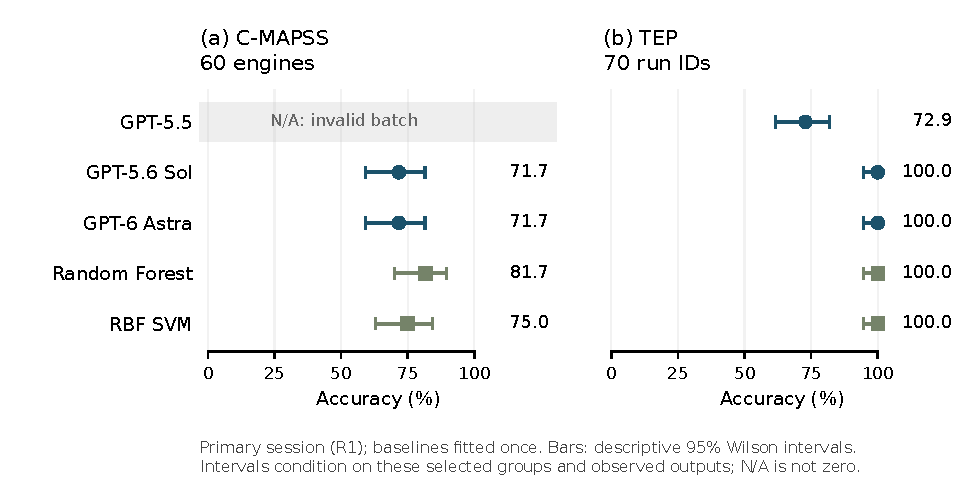
\includegraphics[width=\linewidth]{figures/revision_v3/primary_accuracy.pdf}
\caption{Original-study primary clean-input accuracy with 95\% Wilson intervals on the common test observations. N/A denotes the failed whole-batch response. LLM values use repeat 1; RF and SVM are each fit once. Intervals use the independent-source-unit approximation and are conditional on the observed grouped responses. The training-majority references are given in Table~\ref{tab:primary}.}
\label{fig:primary}
\end{figure}

\subsection{Sensitivity to the mapping intervention}
\begin{table}[htbp]
\centering
\small
\caption{Paired TEP mapping stress test, repeat 1. Accuracy and differences are in percent and percentage points, respectively. Positive differences favor clean inputs. Intervals resample paired source groups conditional on the fixed batch responses. Flips count changes in predicted labels.}
\label{tab:paired}
\begin{tabular}{@{}lrrrrr@{}}
\toprule
Model & Clean & Corrupted & $\Delta$ acc. & 95\% paired interval & Flips \\
\midrule
GPT-5.5 & 72.9 & 44.3 & 28.6 & [11.4, 45.7] & 50/70 \\
GPT-5.6 Sol & 100.0 & 22.9 & 77.1 & [67.1, 87.1] & 54/70 \\
GPT-6 Astra & 100.0 & 100.0 & 0.0 & [0.0, 0.0] & 0/70 \\
\bottomrule
\end{tabular}
\end{table}


Table~\ref{tab:paired} shows the primary paired contrast, while Figure~\ref{fig:mapping} places it alongside the repeated effects and prediction flips. For GPT-5.5, macro F1 changes from 72.1\% to 37.9\% under the descriptor rotation (clean-minus-corrupted difference 34.2 pp). For GPT-5.6 Sol, macro F1 changes from 100.0\% to 22.9\% under the descriptor rotation (clean-minus-corrupted difference 77.1 pp). For GPT-6 Astra, macro F1 changes from 100.0\% to 100.0\% under the descriptor rotation (clean-minus-corrupted difference 0.0 pp). Full accuracy, F1, flip-rate intervals, and all repeated paired contrasts are retained in the machine-readable analysis.

\begin{figure}[htbp]
\centering
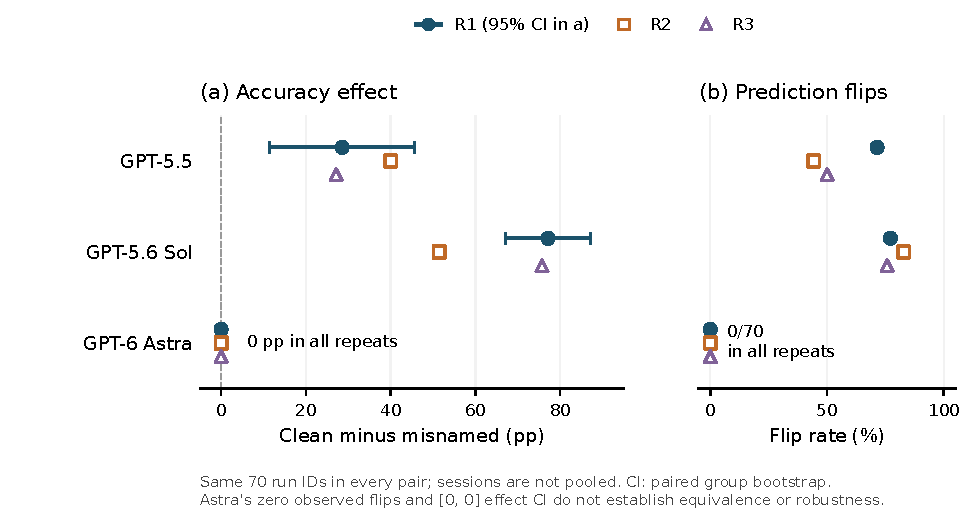
\includegraphics[width=\linewidth]{figures/revision_v3/mapping_sensitivity.pdf}
\caption{TEP sensitivity to the fixed descriptor rotation. Left: clean-minus-corrupted accuracy differences, with paired group-bootstrap 95\% intervals for repeat 1 and separate points for repeats 2 and 3. Right: the proportion of labels that change between paired conditions in each repeat. All comparisons use the same 70 runs; repetitions are separate sessions. Zero effect and zero flips for Astra describe this input set, not equivalence under other corruptions.}
\label{fig:mapping}
\end{figure}

Prediction disagreement is distinct from accuracy change. A mapping fault may replace one wrong label with another, or produce offsetting improvements and degradations. We therefore report both paired score differences and the fraction of observations whose predicted label changes. Neither a small net accuracy change nor a large number of flips, considered alone, establishes physically grounded reasoning.

\subsection{Repeated-session variation and operational error types}
\begin{table}[htbp]
\centering
\small
\caption{Accuracy (\%) for scheduled fresh sessions with identical within-condition payloads. Range is maximum minus minimum over the valid sessions, in percentage points. Valid gives their count. N/A is retained for failed validation; repetitions do not increase the held-out sample size.}
\label{tab:repeat}
\begin{tabular}{@{}llrrrrr@{}}
\toprule
Task/condition & Model & R1 & R2 & R3 & Range & Valid \\
\midrule
C-MAPSS clean & GPT-5.5 & N/A & 68.3 & 66.7 & 1.7 & 2 \\
C-MAPSS clean & GPT-5.6 Sol & 71.7 & 68.3 & 70.0 & 3.3 & 3 \\
C-MAPSS clean & GPT-6 Astra & 71.7 & 73.3 & 75.0 & 3.3 & 3 \\
TEP clean & GPT-5.5 & 72.9 & 80.0 & 57.1 & 22.9 & 3 \\
TEP clean & GPT-5.6 Sol & 100.0 & 70.0 & 100.0 & 30.0 & 3 \\
TEP clean & GPT-6 Astra & 100.0 & 100.0 & 100.0 & 0.0 & 3 \\
TEP corrupted & GPT-5.5 & 44.3 & 40.0 & 30.0 & 14.3 & 3 \\
TEP corrupted & GPT-5.6 Sol & 22.9 & 18.6 & 24.3 & 5.7 & 3 \\
TEP corrupted & GPT-6 Astra & 100.0 & 100.0 & 100.0 & 0.0 & 3 \\
\bottomrule
\end{tabular}
\end{table}


The available model--condition accuracy ranges span 0.0--30.0 pp. Ranges based on two valid sessions should not be compared with three-session ranges as a stability ranking. These are observed ranges across three sessions, not confidence intervals over the service's future behavior. A stable aggregate score may still conceal different sample-level decisions. Figure~\ref{fig:repeat} displays all available scheduled-session accuracies alongside the common-test baselines. Across the 25 valid within-condition pairs of repeated sessions, prediction disagreement ranges from 0.0\% to 42.9\%. These compare repeated predictions of the same observations; they are distinct from the clean-versus-corrupted flips in Table~\ref{tab:paired}.

\begin{table}[htbp]
\centering
\small
\caption{Operational error summaries for clean inputs, repeat 1 for LLMs. C-MAPSS miss means a Critical engine assigned either other class. TEP miss means a fault assigned Normal; false alarm means a Normal observation assigned a fault. These denominators differ from overall accuracy.}
\label{tab:errors}
\begin{tabular}{@{}lrrrrr@{}}
\toprule
Method & Critical miss & Rate (\%) & Fault miss & Rate (\%) & False alarm \\
\midrule
GPT-5.5 & N/A & N/A & 1/60 & 1.7 & 0/10 \\
GPT-5.6 Sol & 2/20 & 10.0 & 0/60 & 0.0 & 0/10 \\
GPT-6 Astra & 5/20 & 25.0 & 0/60 & 0.0 & 0/10 \\
Random Forest & 6/20 & 30.0 & 0/60 & 0.0 & 0/10 \\
RBF SVM & 10/20 & 50.0 & 0/60 & 0.0 & 0/10 \\
\bottomrule
\end{tabular}
\end{table}


Table~\ref{tab:errors} separates fault-to-Normal errors from confusion among fault types; Figure~\ref{fig:recall} shows all class-level recalls. Only ten Normal TEP observations and twenty Critical C-MAPSS engines enter the respective class-specific denominators. Their intervals and full confusion matrices are provided with the analysis; zero observed misses in this subset should not be interpreted as a safety guarantee. Overall accuracy and Critical recall need not rank methods identically: GPT-5.6 Sol misses 2/20 Critical engines, compared with 6/20 for RF in the primary comparison. This small class-specific result is descriptive and does not establish a safety advantage.

The mapping intervention can have opposite effects across fault classes. In GPT-5.5's primary responses, Fault 2 recall changes from 0/10 to 10/10 under the rotation, even though overall accuracy falls. This descriptive pattern helps explain why net accuracy change and prediction disagreement are complementary. The case exports retain each transition for follow-up analysis.

\begin{figure}[htbp]
\centering
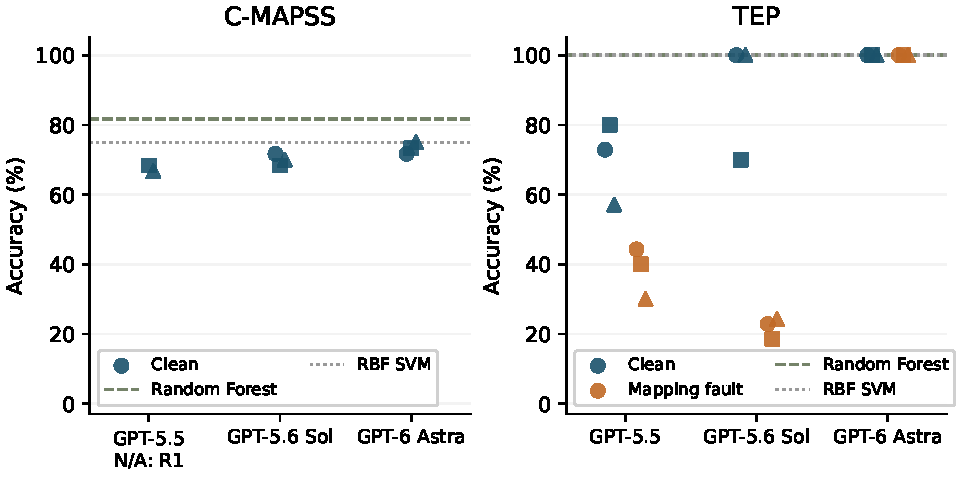
\includegraphics[width=\linewidth]{figures/revision_v3/repeat_accuracy.pdf}
\caption{All available scheduled-session accuracies (circles, squares, triangles for repeats 1, 2, 3). N/A marks the failed batch. Points may overlap. Horizontal lines show the common-test RF and SVM baselines. Their TEP lines coincide. This plot shows repeated scores, not independent test replications.}
\label{fig:repeat}
\end{figure}

\begin{figure}[htbp]
\centering
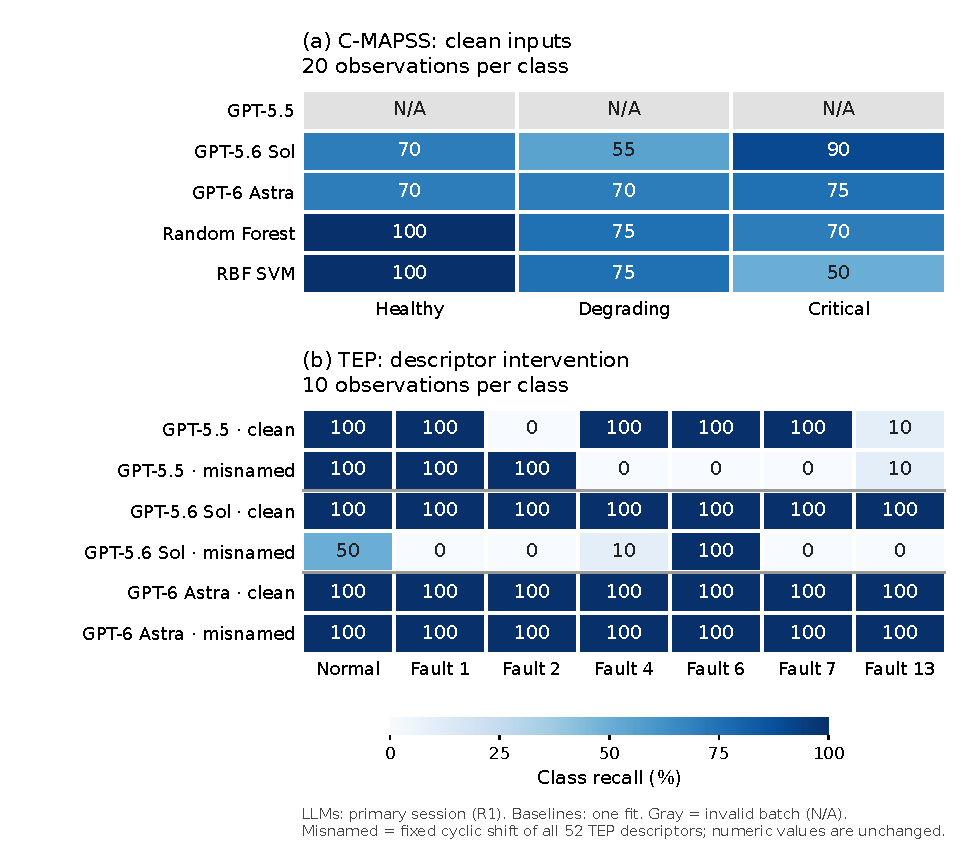
\includegraphics[width=0.85\linewidth]{figures/revision_v3/class_recall.pdf}
\caption{Descriptive class-level recall from the frozen primary responses. Cells show recall (\%); supports are 20 engines per C-MAPSS category and 10 runs per TEP condition. N/A retains the invalid C-MAPSS batch. The paired TEP rows compare clean and rotated-descriptor conditions. Small class denominators make these error profiles exploratory; full confusion counts and intervals are supplied with the analysis.}
\label{fig:recall}
\end{figure}

\FloatBarrier
\subsection{Exploratory representation and context extension}
The separate extension retains all 84 scheduled requests: 84 are valid, yielding 2604 labels eligible for scoring from 2604 requested classifications. These calls concern the same 70 runs as the original TEP comparison. Table~\ref{tab:extension} reports all full-batch repeats, and Table~\ref{tab:context} reports the fixed seven-case context probes.

\begin{table}[htbp]
\centering\small
\caption{Separate exploratory extension on the same 70 TEP runs. Each accuracy column is a fresh full-batch response. Flips compare that condition with the contemporaneous clean response in repeat 1 after ID alignment; N/A retains invalid requests.}
\label{tab:extension}
\begin{tabular}{@{}llrrrr@{}}
\toprule
Model & Condition & R1 (\%) & R2 (\%) & R3 (\%) & R1 flips \\
\midrule
GPT-5.6 Sol & Clean & 100.0 & 100.0 & 100.0 & -- \\
GPT-5.6 Sol & Cyclic mapping fault & 24.3 & 52.9 & 21.4 & 53/70 \\
GPT-5.6 Sol & Correct pair reordering & 100.0 & 71.4 & 57.1 & 0/70 \\
GPT-5.6 Sol & Anonymous fields & 100.0 & 94.3 & 100.0 & 0/70 \\
GPT-5.6 Sol & Random mapping fault & 50.0 & 55.7 & 52.9 & 35/70 \\
GPT-5.6 Sol & Sample reordering & 100.0 & 100.0 & 98.6 & 0/70 \\
\addlinespace
GPT-6 Astra & Clean & 100.0 & 100.0 & 100.0 & -- \\
GPT-6 Astra & Cyclic mapping fault & 100.0 & 100.0 & 100.0 & 0/70 \\
GPT-6 Astra & Correct pair reordering & 100.0 & 100.0 & 100.0 & 0/70 \\
GPT-6 Astra & Anonymous fields & 100.0 & 100.0 & 100.0 & 0/70 \\
GPT-6 Astra & Random mapping fault & 100.0 & 100.0 & 100.0 & 0/70 \\
GPT-6 Astra & Sample reordering & 100.0 & 100.0 & 100.0 & 0/70 \\
\bottomrule
\end{tabular}
\end{table}

GPT-5.6 Sol has fresh clean repeat-1 accuracy of 100.0\%. For correct pair reordering, anonymous fields, random mapping and sample reordering, the corresponding accuracies are 100.0, 100.0, 50.0, 100.0\%, respectively. The respective paired flip counts are 0/70, 0/70, 35/70, 0/70.

GPT-6 Astra has fresh clean repeat-1 accuracy of 100.0\%. For correct pair reordering, anonymous fields, random mapping and sample reordering, the corresponding accuracies are 100.0, 100.0, 100.0, 100.0\%, respectively. The respective paired flip counts are 0/70, 0/70, 0/70, 0/70.

\begin{table}[htbp]
\centering\small
\caption{Seven-case context probe. Entries are prediction flips over available paired cases; the same IDs are used in all three request configurations. Each repeat of the singleton panel consists of seven separate sessions. These small, label-independently selected probes do not estimate general batch-size effects.}
\label{tab:context}
\begin{tabular}{@{}llrrr@{}}
\toprule
Model & Comparison & R1 & R2 & R3 \\
\midrule
GPT-5.6 Sol & 70-record vs. 7-record & 5/7 & 5/7 & 5/7 \\
GPT-5.6 Sol & 7-record vs. single-record & 3/7 & 2/7 & 4/7 \\
GPT-5.6 Sol & 70-record vs. single-record & 3/7 & 3/7 & 4/7 \\
GPT-6 Astra & 70-record vs. 7-record & 1/7 & 1/7 & 1/7 \\
GPT-6 Astra & 7-record vs. single-record & 0/7 & 0/7 & 1/7 \\
GPT-6 Astra & 70-record vs. single-record & 1/7 & 1/7 & 2/7 \\
\bottomrule
\end{tabular}
\end{table}

GPT-5.6 Sol: on the same seven focal records, the full-batch correct counts are 7/7, 7/7, 7/7; seven-record counts are 2/7, 2/7, 2/7; and single-record counts are 4/7, 4/7, 3/7, in repeats 1, 2 and 3 respectively. GPT-6 Astra: on the same seven focal records, the full-batch correct counts are 7/7, 7/7, 7/7; seven-record counts are 6/7, 6/7, 6/7; and single-record counts are 6/7, 6/7, 5/7, in repeats 1, 2 and 3 respectively. The label-free selection contains Fault\_2 (3), Fault\_4 (1), Fault\_6 (2), Fault\_13 (1). Normal and several fault classes are absent. The probe therefore characterizes these seven records rather than class-balanced diagnostic performance. Figure~\ref{fig:matchedcontext} displays the matched correct counts.

All pairwise accuracy differences, conditional intervals and session-level outputs are retained in the extension package. Differences between this extension and the historical sessions are not treated as causal effects of a transformation; each contrast uses its own fresh clean reference.

\begin{figure}[htbp]
\centering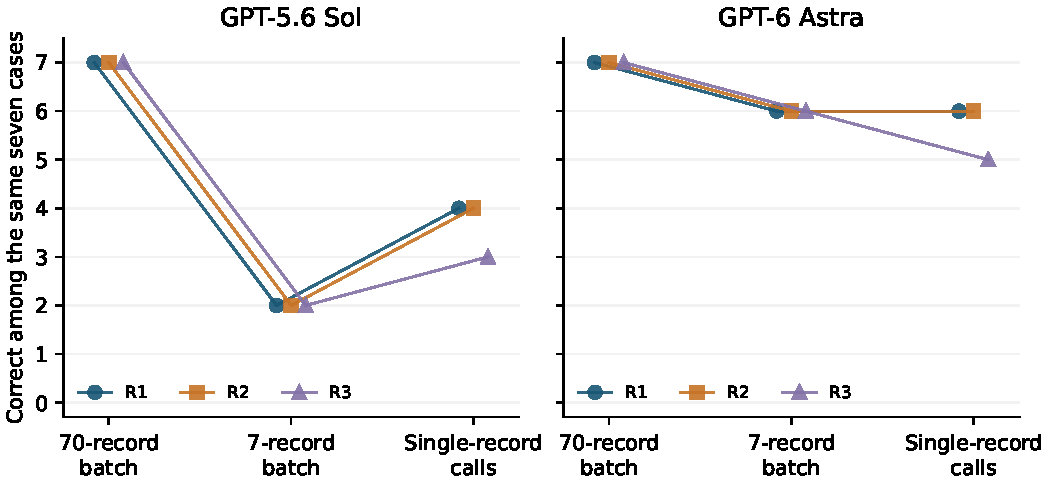
\includegraphics[width=\linewidth]{figures/mechanism_extension/matched_context.pdf}
\caption{Matched context probe on the same seven observations. Each point counts correct predictions for those seven IDs, including when they appear inside the 70-record batch. Horizontal offsets separate the three fresh repetitions; lines connect request configurations and do not imply a continuous size-response law. Single-record points summarize seven separate calls. No new source observations are introduced.}
\label{fig:matchedcontext}\end{figure}


\FloatBarrier
\subsection{Cross-provider coverage and mapping sensitivity}
The revised addition produces 15/18 valid responses and 990/1,200 scorable classifications. DeepSeek yields 7/9 valid batches and Qwen 8/9. All three invalid batches occur under TEP descriptor corruption: DeepSeek repeats 1 and 3 exhaust the 65,536-token completion budget with a length finish; Qwen repeat 2 finishes normally but adds prose before the requested JSON array. The latter is a response-contract failure, and its apparent labels are not extracted or scored. Coverage and accuracy therefore describe different outcomes.

\begin{table}[htbp]
\centering
\small
\caption{Cross-provider addition, repeat 1. Accuracy and macro F1 are percentages; accuracy intervals are 95\% Wilson summaries conditional on the observed grouped response. N/A denotes a failed whole batch. The same RF/SVM references in Table~
ef{tab:primary} apply.}
\label{tab:domestic_primary}
\begin{tabular}{@{}llrrr@{}}
\toprule
Service & Task/condition & Acc. & 95\% interval & Macro F1 \\
\midrule
DeepSeek V4 Pro & C-MAPSS & 66.7 & [54.1, 77.3] & 66.5 \\
DeepSeek V4 Pro & TEP clean & 62.9 & [51.1, 73.2] & 57.4 \\
DeepSeek V4 Pro & TEP corrupted & N/A & N/A & N/A \\
Qwen3.8 Max & C-MAPSS & 53.3 & [40.9, 65.4] & 50.1 \\
Qwen3.8 Max & TEP clean & 42.9 & [31.9, 54.5] & 33.5 \\
Qwen3.8 Max & TEP corrupted & 20.0 & [12.3, 30.8] & 12.3 \\
\bottomrule
\end{tabular}
\end{table}

DeepSeek's primary clean accuracies are 66.7\% on C-MAPSS and 62.9\% on TEP; the corresponding Qwen values are 53.3\% and 42.9\%. For Qwen, the primary clean-minus-corrupted TEP accuracy difference is 22.9 pp (paired bootstrap 95\% interval [14.3, 32.9]); 17/70 labels change. DeepSeek's primary paired contrast remains N/A.

\begin{table}[htbp]
\centering
\small
\caption{All revised API sessions: accuracy (\%) and valid-batch counts. Repeats use the same sources and do not increase sample size. No failed response is scored, repaired, or replaced; one available value cannot establish repeatability.}
\label{tab:domestic_repeat}
\begin{tabular}{@{}llrrrr@{}}
\toprule
Service & Task/condition & R1 & R2 & R3 & Valid \\
\midrule
DeepSeek V4 Pro & C-MAPSS & 66.7 & 66.7 & 61.7 & 3/3 \\
DeepSeek V4 Pro & TEP clean & 62.9 & 74.3 & 34.3 & 3/3 \\
DeepSeek V4 Pro & TEP corrupted & N/A & 15.7 & N/A & 1/3 \\
Qwen3.8 Max & C-MAPSS & 53.3 & 61.7 & 60.0 & 3/3 \\
Qwen3.8 Max & TEP clean & 42.9 & 51.4 & 44.3 & 3/3 \\
Qwen3.8 Max & TEP corrupted & 20.0 & N/A & 37.1 & 2/3 \\
\bottomrule
\end{tabular}
\end{table}

DeepSeek's clean TEP accuracy ranges from 34.3\% to 74.3\% across the three valid repeats, a 40.0-pp range. Its only valid corrupted batch is repeat 2; the matched accuracy difference is 58.6 pp (95\% interval [45.7, 70.0]). Qwen's second available pair, repeat 3, differs by 7.1 pp. These secondary contrasts retain their repeat identities. Full macro-F1 intervals, class-level confusion matrices, paired differences and case records accompany the tables.
\FloatBarrier

\subsection{Usable correct outputs across scheduled requests}
Table~\ref{tab:usable} adds descriptive delivery accounting to the original and revised API schedules. Each cell covers three scheduled batches on the same source units. Repeated classifications are counted as delivery opportunities, not independent observations. The representation/context follow-up has a different schedule and is not mixed into this comparison. The table is not an equal-compute ranking.

\begin{table}[htbp]
\centering\small
\caption{Post hoc delivery accounting across the three scheduled repeats. Valid counts whole batches. $C/V$ counts correct labels within valid output; $A_{\mathrm{valid}}$ and $Y$ are percentages. For $Y$, the denominator is 180 scheduled slots for C-MAPSS and 210 for each TEP condition. Invalid batches remain N/A in classification tables and contribute no usable correct outputs here.}
\label{tab:usable}
\begin{tabular}{@{}llrrrr@{}}
\toprule
Service & Task/condition & Valid & $C/V$ & $A_{\mathrm{valid}}$ & $Y$ \\
\midrule
GPT-5.5 & C-MAPSS & 2/3 & 81/120 & 67.5 & 45.0 \\
GPT-5.5 & TEP clean & 3/3 & 147/210 & 70.0 & 70.0 \\
GPT-5.5 & TEP corrupted & 3/3 & 80/210 & 38.1 & 38.1 \\
GPT-5.6 Sol & C-MAPSS & 3/3 & 126/180 & 70.0 & 70.0 \\
GPT-5.6 Sol & TEP clean & 3/3 & 189/210 & 90.0 & 90.0 \\
GPT-5.6 Sol & TEP corrupted & 3/3 & 46/210 & 21.9 & 21.9 \\
GPT-6 Astra & C-MAPSS & 3/3 & 132/180 & 73.3 & 73.3 \\
GPT-6 Astra & TEP clean & 3/3 & 210/210 & 100.0 & 100.0 \\
GPT-6 Astra & TEP corrupted & 3/3 & 210/210 & 100.0 & 100.0 \\
DeepSeek V4 Pro & C-MAPSS & 3/3 & 117/180 & 65.0 & 65.0 \\
DeepSeek V4 Pro & TEP clean & 3/3 & 120/210 & 57.1 & 57.1 \\
DeepSeek V4 Pro & TEP corrupted & 1/3 & 11/70 & 15.7 & 5.2 \\
Qwen3.8 Max & C-MAPSS & 3/3 & 105/180 & 58.3 & 58.3 \\
Qwen3.8 Max & TEP clean & 3/3 & 97/210 & 46.2 & 46.2 \\
Qwen3.8 Max & TEP corrupted & 2/3 & 40/140 & 28.6 & 19.0 \\
\bottomrule
\end{tabular}
\end{table}

DeepSeek V4 Pro supplies 11 correct labels in 70 validated corrupted-TEP slots (15.7\% conditional accuracy), compared with 210 scheduled slots (5.2\% usable correct output). 
Qwen3.8 Max supplies 40 correct labels in 140 validated corrupted-TEP slots (28.6\% conditional accuracy), compared with 210 scheduled slots (19.0\% usable correct output). 
This difference quantifies delivered output under the specified whole-batch contract. It does not impute the unobserved correctness of failed responses or measure fault-alarm utility, and it depends on the chosen validation and retry rules.

\FloatBarrier

\subsection{Source-disjoint follow-up: mapping, context and transfer}
The fourth stage yields 84/84 valid responses and 4,854/4,854 eligible labels. All scheduled outcomes are retained. Tables~\ref{tab:ind_mapping}--\ref{tab:ind_transfer} show the planned conditions; Figure~\ref{fig:independent} summarizes their repeated outcomes. All comparisons below use the new source panel, separately from the preceding discovery stages.

\begin{table}[htbp]
\centering
\small
\caption{New TEP main panel (70 runs). Accuracy for each scheduled repeat and primary macro F1 are percentages. Primary flips compare the condition with its contemporaneous clean response. Correct-pair reordering is a physically matched control, not an incorrect mapping.}
\label{tab:ind_mapping}
\begin{tabular}{@{}llrrrrr@{}}
\toprule
Service & Condition & R1 & R2 & R3 & R1 F1 & R1 flips \\
\midrule
5.6 Sol & Clean & 100.0 & 97.1 & 100.0 & 100.0 & -- \\
5.6 Sol & Rotation & 32.9 & 62.9 & 25.7 & 33.6 & 47/70 \\
5.6 Sol & Random 1 & 100.0 & 100.0 & 40.0 & 100.0 & 0/70 \\
5.6 Sol & Random 2 & 97.1 & 68.6 & 100.0 & 97.1 & 2/70 \\
5.6 Sol & Random 3 & 62.9 & 100.0 & 97.1 & 62.9 & 26/70 \\
5.6 Sol & Same-unit swap & 98.6 & 100.0 & 71.4 & 98.6 & 1/70 \\
5.6 Sol & Correct-pair reorder & 100.0 & 97.1 & 100.0 & 100.0 & 0/70 \\
6 Astra & Clean & 100.0 & 100.0 & 100.0 & 100.0 & -- \\
6 Astra & Rotation & 100.0 & 100.0 & 100.0 & 100.0 & 0/70 \\
6 Astra & Random 1 & 100.0 & 100.0 & 100.0 & 100.0 & 0/70 \\
6 Astra & Random 2 & 100.0 & 100.0 & 100.0 & 100.0 & 0/70 \\
6 Astra & Random 3 & 100.0 & 100.0 & 100.0 & 100.0 & 0/70 \\
6 Astra & Same-unit swap & 100.0 & 100.0 & 100.0 & 100.0 & 0/70 \\
6 Astra & Correct-pair reorder & 100.0 & 100.0 & 100.0 & 100.0 & 0/70 \\
\bottomrule
\end{tabular}
\end{table}
For GPT-5.6 Sol, the primary clean-to-rotation accuracy difference is 67.1 pp (conditional 95\% interval [55.7, 78.6]); primary accuracies across the three random mappings span 62.9--100.0\%. For GPT-6 Astra, the primary clean-to-rotation accuracy difference is 0.0 pp (conditional 95\% interval [0.0, 0.0]); primary accuracies across the three random mappings span 100.0\%. These finite realizations do not estimate a distribution over all mapping errors.

\begin{table}[htbp]
\centering
\small
\caption{The same 21 new focal observations in six contexts, covering all seven classes. Cells give correct focal labels, not whole-request accuracy. Parentheses denote total request size; the additional cases in A/B are not included in the numerator.}
\label{tab:ind_context}
\begin{tabular}{@{}llrrr@{}}
\toprule
Service & Focal context & R1 & R2 & R3 \\
\midrule
5.6 Sol & Within clean (70) & 21/21 & 19/21 & 21/21 \\
5.6 Sol & Focal only (21) & 21/21 & 21/21 & 15/21 \\
5.6 Sol & Focal before A (42) & 21/21 & 21/21 & 13/21 \\
5.6 Sol & Focal after A (42) & 21/21 & 20/21 & 21/21 \\
5.6 Sol & Focal before B (42) & 21/21 & 15/21 & 21/21 \\
5.6 Sol & Focal after B (42) & 9/21 & 15/21 & 15/21 \\
6 Astra & Within clean (70) & 21/21 & 21/21 & 21/21 \\
6 Astra & Focal only (21) & 20/21 & 20/21 & 20/21 \\
6 Astra & Focal before A (42) & 21/21 & 20/21 & 20/21 \\
6 Astra & Focal after A (42) & 20/21 & 20/21 & 20/21 \\
6 Astra & Focal before B (42) & 21/21 & 20/21 & 20/21 \\
6 Astra & Focal after B (42) & 21/21 & 21/21 & 21/21 \\
\bottomrule
\end{tabular}
\end{table}
Across the six prespecified comparisons of each type (two per repeat), GPT-5.6 Sol shows 0--12 out of 21 for background and 0--12 out of 21 for position label flips. GPT-6 Astra shows 0--1 out of 21 for background and 0--1 out of 21 for position label flips. These comparisons vary one context dimension at a time, while repeated calls still include service variability. They do not identify the model's internal mechanism.

\begin{table}[htbp]
\centering
\small
\caption{New-source classification and fixed-representation transfer. LLM accuracy lists R1/R2/R3; RF/SVM are each fit once on original training data. F1 and Wilson intervals use R1 for LLMs. All values are percentages; intervals are conditional independent-unit approximations. Earlier TEP shares the 70 late-stage runs; FD002 has 60 different engines.}
\label{tab:ind_transfer}
\begin{tabular}{@{}llrrr@{}}
\toprule
Panel & Method & Acc. (R1/R2/R3) & R1 F1 & R1 95\% interval \\
\midrule
TEP late & 5.6 Sol & 100.0/97.1/100.0 & 100.0 & [94.8, 100.0] \\
TEP late & 6 Astra & 100.0/100.0/100.0 & 100.0 & [94.8, 100.0] \\
TEP late & Random Forest & 100.0 & 100.0 & [94.8, 100.0] \\
TEP late & RBF SVM & 92.9 & 92.6 & [84.3, 96.9] \\
TEP earlier & 5.6 Sol & 87.1/85.7/88.6 & 87.1 & [77.3, 93.1] \\
TEP earlier & 6 Astra & 88.6/87.1/88.6 & 86.4 & [79.0, 94.1] \\
TEP earlier & Random Forest & 28.6 & 21.4 & [19.3, 40.1] \\
TEP earlier & RBF SVM & 31.4 & 25.1 & [21.8, 43.0] \\
FD002 & 5.6 Sol & 60.0/26.7/56.7 & 61.1 & [47.4, 71.4] \\
FD002 & 6 Astra & 71.7/76.7/78.3 & 72.7 & [59.2, 81.5] \\
FD002 & Random Forest & 33.3 & 16.7 & [22.7, 45.9] \\
FD002 & RBF SVM & 33.3 & 16.7 & [22.7, 45.9] \\
\bottomrule
\end{tabular}
\end{table}
No FD002 observation is used to tune channels, preprocessing or classifier hyperparameters. The TEP phase contrast pairs earlier and later snapshots by the same run; their classifications are not pooled as 140 independent sources.

Primary earlier-TEP accuracies are 87.1\% for Sol and 88.6\% for Astra, compared with 28.6\% for RF and 31.4\% for SVM. These baselines are trained on the original late-snapshot representation; this difference is conditional on that training-to-test phase shift, not evidence against earlier-phase-trained classifiers. On FD002, the primary service accuracies are 60.0\% and 71.7\%, while both unadapted baselines give 33.3\%. No optimized regime-aware reference is evaluated.

\begin{figure}[htbp]
\centering
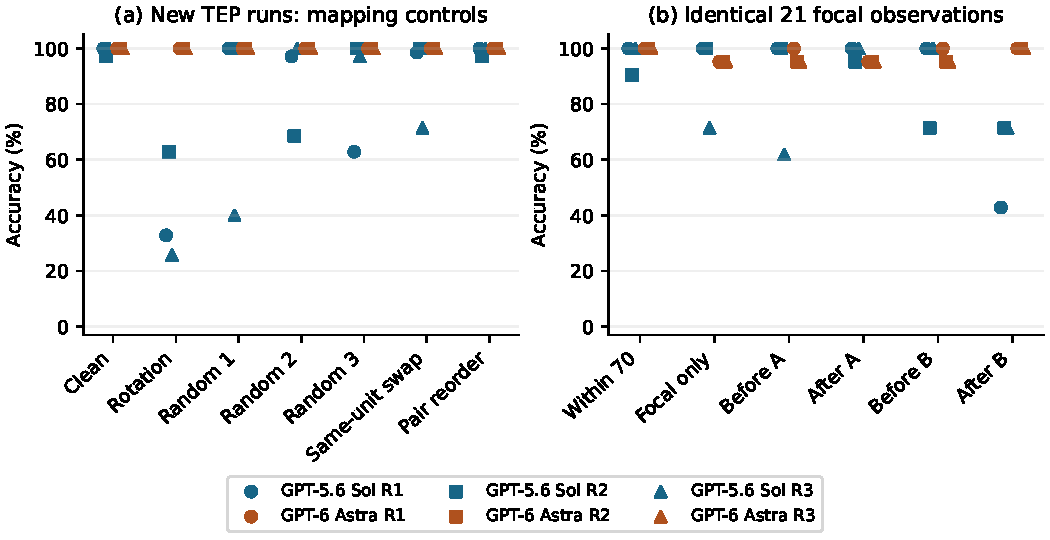
\includegraphics[width=\linewidth]{figures/independent_validation/independent_controls.pdf}
\caption{All three scheduled repeats of the new-source mapping and context panels. Color identifies service; circles, squares and triangles identify repeats 1, 2 and 3. Panel (a) uses 70 new TEP runs per condition. Panel (b) scores only the same 21 focal cases in each request. These repeated points describe observed calls, not confidence intervals or added independent sources.}
\label{fig:independent}
\end{figure}
\FloatBarrier

\section{Discussion}
\subsection{Mapping sensitivity and semantic use are different claims}
The common evaluation set makes differences between LLM and supervised scores directly traceable to the same observations. Source-group separation assesses prediction on held-out engines or simulation runs. The original comparison remains within each benchmark: FD001 uses one operating condition, and TEP test runs share the simulator and selected fault definitions with training. The fourth stage separately examines the fixed FD001 representation on FD002, which contains six operating conditions. Strong supervised performance is therefore compatible with a relatively separable test subset, particularly for the late TEP snapshots.

The paired stress test permits a more specific interpretation than comparing two historical input versions. Samples, values, output format, and class definitions are held fixed, so the planned descriptor rotation is the controlled input difference. Repeated sessions show whether the observed pattern persists across three service calls under this fixed design. They cannot establish that every future run or every possible mapping defect will behave similarly. A robust production interface should validate column identities before inference regardless of whether a model sometimes compensates for the error.

Clean TEP accuracy is at least as high as corrupted accuracy in all nine model--repeat comparisons, with ties in some sessions. The complete contrast set is retained regardless of its direction. The supervised baselines already classify all selected late-stage TEP snapshots correctly, leaving no measured accuracy advantage for the LLM interface on this subset. Its possible advantages in explanation, interaction, or transfer are separate questions that this label-only experiment does not measure.

GPT-6 Astra gives identical clean and corrupted predictions in all three paired repetitions. This contrasts with the responses of the other evaluated services and prevents a claim that the mapping fault universally reduces accuracy. Invariance under an incorrect descriptor mapping also does not prove that descriptors are used correctly. Reliance on retained numerical patterns, canonical variable order, or recognition and compensation for an obvious mapping shift are possible explanations; this experiment does not distinguish them. The result motivates separate tests of value order and individual fields rather than an unsupported claim about internal reasoning or benchmark memorization.

\subsection{What the added controls can discriminate}
At least one repeated response changes for GPT-5.6 Sol under cyclic mapping fault, correct pair reordering, anonymous fields, random mapping fault, sample reordering. GPT-6 Astra shows no observed flips in any of the three paired repetitions for cyclic mapping fault, correct pair reordering, anonymous fields, random mapping fault, sample reordering.

The context probe qualifies the perfect full-batch scores: both services change at least one focal prediction when surrounding records are removed, despite unchanged focal sensor text. The repeated seven-record deficits are especially pronounced for Sol. These observations establish a dependence of observed outcomes on the tested request configuration; context composition, position and stochastic service behavior remain intertwined.

Correct pair reordering preserves the represented physical state, so disagreement under this condition is evidence of sensitivity to presentation for the tested input. Anonymous fields jointly remove sensor identity, name and unit while retaining task-level fault descriptions. Retained accuracy would therefore show that explicit sensor-field descriptors are unnecessary for those decisions in that context, without establishing how the model obtained them. A noncyclic mapping fault tests whether invariance is confined to the original regular rotation, while retaining numerical position as a possible cue. None of these controls alone establishes or excludes benchmark exposure.

The seven-case context comparisons inspect whether a fixed observation receives a different label when surrounding observations change. A nonzero flip count establishes an observed context-associated discrepancy; zero flips in this small probe do not establish sample independence. Shared service stochasticity also contributes to these comparisons. The original sample selection, post hoc model selection and small context panel restrict these findings to hypothesis refinement. The source-disjoint fourth stage addresses the first two gaps with new runs and several mappings; a broader provider sample and external data-generation processes remain necessary for wider generalization.


\subsection{What the cross-provider addition establishes}
The API addition broadens the observed service families and preserves the same numerical cases and descriptor intervention. Its valid pairs show lower accuracy under descriptor corruption, while its incomplete and nonconforming responses expose an additional interface failure. Reporting only valid classification scores would omit that failure. Because missingness occurs under corruption, available paired scores need not represent the outcomes that would have been obtained from every scheduled request; N/A is neither zero accuracy nor evidence of robustness.

This extension does not isolate provider identity as a causal factor. The original services and the API additions differ in transport, instruction role, reasoning controls and potentially hidden service settings. The budget was revised after a configuration failure, and the addition was planned after seeing the original study. It therefore supports exploratory comparisons of recorded service configurations, rather than an equal-compute model ranking. The representation/context controls remain limited to Sol and Astra; their findings cannot be transferred to DeepSeek or Qwen from the present addition alone.

\subsection{What the source-disjoint follow-up adds}
The additional stage addresses two distinct gaps: replicating the interface tests on previously unused simulator runs, and challenging the fixed FD001 representation on a six-operating-condition subset. The 21-case focal panel also includes every selected TEP class, unlike the original seven-case probe. Its crossed A/B and front/back comparisons narrow the context interpretation by holding request size fixed. Nevertheless, each observed contrast contains variation from separate service calls. Three repeats are insufficient to estimate stable average causal effects over prompts, providers or times.

The new focal panel also qualifies the earlier seven-case result: Sol classifies all 21 focal-only cases correctly in the first two repeats, whereas its primary focal score falls to 9/21 when background B precedes them. Thus, fewer accompanying cases do not consistently imply worse classification. Astra retains perfect new full-batch mapping scores but makes one error in each focal-only repeat. These are configuration-specific patterns rather than a universal batch-size law.

Mapping realizations are operationally different interventions. A random reassignment can be less regular than the cyclic rotation; a same-unit local swap changes only two identities; correct-pair reordering preserves physical correspondence. Their separate outcomes qualify any general claim about ``sensor-name robustness.'' The phase and FD002 contrasts likewise characterize the specified snapshot representation rather than early warning, diagnostic reasoning or optimized transfer learning. Any discrepancy from the original results is retained as evidence of scope dependence, not repaired by replacing observations or choosing a later repeat.

\subsection{Execution interface and limits of cross-provider comparison}
A common numerical payload is necessary but insufficient for an interpretable model comparison. Tool availability, inherited project context, input delivery, output validation and missing-result handling can alter the effective task. The separate conversational exploration in Appendix~\ref{app:claude_reported} illustrates this distinction: some saved arrays support an arithmetic comparison, yet complete inference records and pre-score freezing are not established. Those records are therefore not pooled with the controlled results or used to substantiate a model ranking.

Even within the controlled stages, provider-specific system instructions, reasoning settings and service aliases differ. The paired within-service contrasts identify responses to the specified input interventions under the recorded configurations. Cross-service score differences remain comparisons of complete interfaces, not isolated effects of model architecture or training. A next cross-provider study should predefine comparable context construction and logging, retain every failed request, and report the primary repeat separately from repeated-session summaries.

\subsection{Implications for reusable evaluation}
Within the controlled stages, the practical unit of reuse is a traceable observation and its paired responses. Each feature is linked to a named source channel or past-only window, and each prediction to a frozen request and response. The reproduction package supports three uses: rebuilding published scores and plots without inference, studying sample-level disagreements, and evaluating a new model adapter on the same inputs. Table~\ref{tab:reuse} identifies the corresponding artifacts.

A new adapter should preserve the input order, permitted labels and output contract, record its service settings, and write to a separate result version. Failed coverage must remain visible alongside classification scores. Comparisons using single-observation requests, different sample orders or altered prompting answer additional questions and should be reported as separate conditions. The validator checks structure and provenance; adapting the workflow to another plant also requires a domain review of channel identities, units and label definitions.

\begin{table}[htbp]
\centering\small
\caption{Reusable artifacts and the analyses they support. These materials are included in the local reproduction package; public archiving remains a release step.}
\label{tab:reuse}
\begin{tabularx}{\linewidth}{@{}>{\raggedright\arraybackslash}p{0.28\linewidth}>{\raggedright\arraybackslash}X@{}}
\toprule
Artifact & Reuse supported \\
\midrule
Derived features and source manifest & Reconstruct fixed cases and verify engine/run separation and shared numerical inputs. \\
Label-free paired prompts & Evaluate an additional model on unchanged clean and rotated descriptors. \\
JSON contract and validator & Schema checks types and permitted labels; cross-file validation checks ordered coverage, unique IDs and provenance. \\
Frozen responses and case CSVs & Inspect individual errors, clean-to-corrupted transitions and repeated-session disagreement. \\
Figure data and plotting scripts & Rebuild the published visualizations and reanalyze their underlying values. \\
\bottomrule
\end{tabularx}
\end{table}

\subsection{Limitations and next validation steps}
The source evaluation covers two simulated tasks, selected fault classes, balanced test subsets, and five requested service aliases across three provider families. The representation/context and source-disjoint follow-ups evaluate only two services from the original family. The latter broadens the source count and operating-condition coverage, but the other interface conditions reuse observations. It does not test a physical plant, novel fault types, evolving class prevalence, sensor dropout, noise robustness, time-series alarms, or maintenance utility. The RUL categories are retrospective proxies, and even the additional earlier TEP snapshots are 60 minutes after fault injection. Deployment decisions would require calibrated risk, realistic prevalence, chronological evaluation, and an application-specific cost of missed faults.

The original grouped interface permits interactions among observations despite the instruction to classify independently. Three repeats and a small set of context configurations cannot exhaust order, composition or service effects. The original mapping fault is deliberately large and regular. The follow-up adds three fixed random derangements, one same-unit swap and a correct-pair reordering control. These examples do not exhaust plausible schema errors. Physically equivalent unit conversions, unseen fault mechanisms and altered simulator parameters remain untested.

Batch completeness is a separate operational requirement. Our classification tables condition on successful whole-batch validation, so they do not measure end-to-end availability. The incomplete and nonconforming responses show why valid-output coverage must accompany accuracy. A production interface would need a separately evaluated structured-output and failure-recovery policy rather than assuming that every request yields one usable label per observation.

Public benchmark familiarity and undisclosed pretraining prevent us from distinguishing acquired engineering knowledge from exposure to benchmark-specific patterns. Service aliases can change, while hidden base instructions and decoding settings limit exact replay. Request-level provenance and full outputs make these constraints inspectable. The class-level visualizations and case exports are descriptive views of the frozen predictions, added during manuscript development; they introduce no new confirmatory hypotheses. Latency and token usage are operational observations; the differing interfaces, accounting conventions and cache behavior do not support a standardized monetary-cost comparison here.

The remaining external-validity question concerns genuinely new data-generation processes. Additional runs from the same TEP simulator test source replication; FD002 tests a specified operating-condition transfer within C-MAPSS. Neither substitutes for a chronological physical-plant study. The crossed 21-case panel improves class coverage and separates background identity from focal position at a fixed request size, but a larger, independently sampled panel and more service-time blocks would be needed to estimate stable average context effects. A production validation should specify realistic prevalence, acceptable false-alarm and missed-fault costs, and an evaluated recovery policy before deployment.

\section{Conclusion}
On the selected simulated observations, classification success, sensitivity to a descriptor fault and response availability provide distinct assessments of the same language-model interface. The original primary descriptor rotation reduces TEP accuracy by 28.6 and 77.1 percentage points for GPT-5.5 and GPT-5.6 Sol, while GPT-6 Astra preserves its labels in all three original paired sessions. In the separate follow-up, descriptor invariance on the full TEP batch coexists with changed decisions for the same focal records in smaller contexts. This distinguishes observed mapping invariance from context-independent classification and makes request composition an explicit part of the evaluation contract. The separately frozen API addition extends the mapping-sensitivity evidence to other service families while showing that response availability must be reported alongside conditional classification scores. These observations support an evaluation protocol that retains paired decision changes, context controls and failed requests alongside accuracy. The source-disjoint stage extends the evidence to 302 total source units with multiple mappings and crossed focal contexts, while separating within-simulator replication from fixed-representation FD002 transfer. Physical-plant deployment still requires prospective operational validation.

\section*{Data and code availability}
Fixed inputs, prompts, protocols, frozen model outputs, event logs, per-case predictions, baseline code and all analysis scripts for every stage are available at \url{https://github.com/song-ouyang/sci}. The original simulation and test-rig datasets are obtained from the cited sources. All analyses can be rebuilt offline from the frozen outputs without new model requests.

\appendix
\section{Audit controls and historical material}
\begin{table}[htbp]
\centering\small
\caption{Checks in the revised workflow and the failure they address.}
\label{tab:audit}
\begin{tabularx}{\linewidth}{@{}>{\raggedright\arraybackslash}p{0.27\linewidth}>{\raggedright\arraybackslash}X@{}}
\toprule
Check & Failure addressed \\
\midrule
Named source-column extraction & Metadata or reordered columns receiving sensor descriptors by position. \\
Engine/run intersection check & Related observations present on both sides of a split. \\
Past-only, exactly 30-row window & Future values or an unintended 31-cycle interval. \\
Rounded-array/text agreement & Classifier families receiving different numerical precision. \\
Paired ID/value/order check & An input intervention silently changing the evaluated observations. \\
Exact JSON and label validation & Partial coverage, duplicate IDs, and overlapping label substrings. \\
Complete event/response records & Truncation or tool use being mistaken for a valid direct classification. \\
Frozen hashes before scoring & Unrecorded prediction revision after answer inspection. \\
\bottomrule
\end{tabularx}
\end{table}

Historical CWRU experiments, additional model families and earlier prompt variants are retained separately for traceability. Their scores are excluded from the present comparison. Changes between historical versions that also alter sample membership or inference format cannot identify a causal ID effect, and responses parsed by substring cannot establish a general chain-of-thought failure mechanism. The original frozen experiment and its reporting amendment define the original primary evidence; all three follow-ups retain their own protocols and output manifests.

The cross-provider API addition has its own plan, frozen output manifest and separately archived aborted configuration trial. Its native response streams and terminal failures are included in the review package. A historical Claude Agent-tool collection, including a manually regenerated batch read in chunks in an existing conversation, is excluded from the controlled comparisons. The available records do not establish isolated fresh inference, authenticated complete-input delivery, or a pre-score output freeze. Removing an integrity flag or changing a response hash cannot establish those properties. This exclusion concerns provenance and protocol comparability, not a claim that every submitted label is wrong; the artifacts and audit are preserved separately. The following appendix distinguishes the corrected historical summary from the later tool-enabled conversational exploration and reports their unresolved provenance limits.

\FloatBarrier
\section{Claude records outside the controlled comparisons}
\label{app:claude_reported}
\subsection{Historical collection and corrected arithmetic}
An earlier collection contains 27 arrays under caller-written Sonnet, Opus and Fable identifiers. A retrospective arithmetic check reproduces its supplied means, but only 23/27 local artifact chains are internally consistent; none has sufficient evidence for inclusion in the controlled comparison. The record labelled Fable uses the invocation alias \texttt{opus}, without a verified service-returned identity. It cannot establish a third distinct tested model. The updated Fable corrupted-condition accuracies are 91.4\%, 95.7\% and 100.0\% (mean 95.7\%, sample SD 4.3 percentage points), correcting the earlier report of three perfect results. The original reported summaries and the subsequent correction are retained in separate audit snapshots. These post-score copies do not establish a prediction freeze before scoring.

\subsection{Separate tool-enabled conversational exploration}
A later exploration specifies 18 records: the requested \texttt{sonnet} and \texttt{opus} aliases, three conditions and three repeats. It reuses the original 60 C-MAPSS engines and 70 TEP runs. The organizer reports using Claude Code desktop Agent calls, with agents loading the prompt files through the Read tool. This is a tool-enabled conversational workflow, not the text-only, tool-disabled interface of the four controlled stages. Exact server-resolved model versions and exclusion of inherited context have not been verified.

The submitted directory contains 16 complete ID sets and two recorded failures: Sonnet corrupted R2 returned an off-task orchestration message, and Opus corrupted R3 returned 69/70 records. Their partial or off-task outputs are not scored. An additional format check finds that Sonnet clean R1 swaps the records at positions 17 and 18 despite the prompt's exact-order requirement. Consequently, 15/18 arrays satisfy the output contract, covering 990/1,200 planned labels. This is structural coverage only; it does not certify execution provenance. Table~\ref{tab:claude_conversation} reports descriptive statistics for those arrays.

\begin{table}[htbp]
\centering
\small
\caption{Tool-enabled conversational records: descriptive scores of arrays satisfying the exact-order output contract. Means and sample SDs (denominator $n-1$) are computed from unrounded session scores; accuracy and macro F1 are on a percentage scale. Available/planned counts describe output structure, not verified inference provenance. All records remain outside the controlled comparisons.}
\label{tab:claude_conversation}
\begin{tabular}{@{}lllrr@{}}
\toprule
Requested alias & Condition & Available & Accuracy & Macro F1 \\
\midrule
Sonnet alias & C-MAPSS & 3/3 & $63.3 \pm 6.7$ & $63.5 \pm 7.1$ \\
Sonnet alias & TEP clean & 2/3 & $65.7 \pm 6.1$ & $62.5 \pm 10.6$ \\
Sonnet alias & TEP corrupted & 2/3 & $16.4 \pm 1.0$ & $9.9 \pm 2.6$ \\
Opus alias & C-MAPSS & 3/3 & $64.4 \pm 1.0$ & $65.0 \pm 1.0$ \\
Opus alias & TEP clean & 3/3 & $100.0 \pm 0.0$ & $100.0 \pm 0.0$ \\
Opus alias & TEP corrupted & 2/3 & $100.0 \pm 0.0$ & $100.0 \pm 0.0$ \\
\bottomrule
\end{tabular}
\end{table}


For transparency, a separate post-hoc ID-aligned calculation includes the complete but misordered Sonnet clean R1 array, without changing its saved bytes or protocol status. Under that sensitivity calculation, the Sonnet clean mean is 64.8\% (sample SD 4.6 percentage points; three arrays), and macro F1 is 61.1\% (sample SD 7.9). This recovers the supplied descriptive summary and raises arithmetically usable coverage to 1,060/1,200 labels; it is not an alternative success definition chosen for the main study.

\begin{table}[htbp]
\centering
\small
\caption{Matched-repeat contrasts for the separate conversational records. Delta is corrupted minus clean accuracy in percentage points. Only repeats with both arrays available enter each contrast. The post-hoc ID-aligned audit includes one complete but misordered Sonnet array; it does not repair the stored response or retrospectively waive its output-contract failure. Repeats reuse the same 70 runs.}
\label{tab:claude_conversation_pairs}
\begin{tabular}{@{}llllr@{}}
\toprule
Analysis & Requested alias & Pairs & $\Delta$ (pp) & Label flips \\
\midrule
Exact order & Sonnet alias & R3 & -45.7 & 37/70 \\
Exact order & Opus alias & R1, R2 & 0.0 & 0/70, 0/70 \\
ID-aligned audit & Sonnet alias & R1, R3 & -45.7 & 47/70, 37/70 \\
ID-aligned audit & Opus alias & R1, R2 & 0.0 & 0/70, 0/70 \\
\bottomrule
\end{tabular}
\end{table}


The supplied 48.4-percentage-point Sonnet decrease subtracts means over different repeat sets. When the ID-aligned analysis uses R1 and R3 on both sides, clean and corrupted means are 62.1\% and 16.4\%, respectively: a 45.7-point decrease, with 47/70 and 37/70 label changes. The exact-order analysis retains only R3, with the same observed decrease but only one paired repeat. For the Opus alias, R1 and R2 each have perfect scores and zero paired label changes; corrupted R3 is unavailable. Neither two equal scores nor zero observed flips establishes deterministic inference, general robustness, or absence of descriptor use.

\subsection{Provenance limits and interpretation}
The submitted scorer labels the two documented failures as \texttt{not\_run}, while the session registry still labels all 18 jobs as running. The audit retains those original files and supplies a separate corrected terminal-status table. The submitted prompt hashes match the current files' MD5 digests; the audit additionally records SHA-256. Current-file agreement does not establish what each agent actually received. Complete original inputs, Read return contents, response transcripts and a prediction manifest demonstrably predating scoring are absent from the supplied directory. The off-task response mentions other agents and a retry, but without the underlying transcript this does not establish which additional calls occurred or whether their outputs entered another record.

Accordingly, these records are reported only as exploratory observations with unresolved execution provenance. They neither enlarge the four-stage request/source totals nor support a controlled cross-provider effect estimate. The observed Sonnet changes motivate further testing of this descriptor intervention; they do not quantify reliance on names or identify an internal mechanism. Opus invariance in the two available pairs is a property of those saved responses. Missingness, tools, inherited context, service identity and input delivery remain possible explanations that cannot be separated here. Retrospective arithmetic verification is distinct from prospective experiment validation.


\FloatBarrier
\section*{AI-assisted preparation}
OpenAI Codex and Anthropic Claude were used to assist with analysis-code maintenance, consistency checks and language editing. The author reviewed all content and takes full responsibility for it. The LLM services evaluated in the study are described in the main text.
\section{Measured follow-up and repeated-input reanalysis}
This appendix was added after the archived four-stage report above. Its hydraulic results are a separate exploratory study; they do not retrospectively amend the original protocols or turn measured cycles into independent devices. The focused manuscript provides the new sampling and execution methods. The local package retains every condition, timestamp, response, failure and per-case score.

\subsection{Hydraulic outcomes and input contract}
The measured schedule yields 29/63 valid requests and 585/1,278 valid classification slots, separately from the four simulation stages. Two requests time out after network disconnections; the stopping rule leaves 32 unattempted. Only R1 and R2 are complete; R3 is partial and R4--R5 are unattempted. Each failed job has one invocation, within which native transport reconnections are recorded. Primary fixed-focal, intact-reorder and descriptor-rotation results are 6/18, 16/18 and 8/18, respectively (Table~\ref{tab:hydraulic}). 

\begin{table}[htbp]\centering\small
\caption{Measured hydraulic follow-up: correct labels among the same 18 focal cycles. R1--R5 are scheduled execution blocks, not independent devices. All planned repetitions are shown; N/A denotes an invalid or unattempted request.}
\label{tab:hydraulic}
\begin{tabular}{@{}lrrrrr@{}}\toprule
Input condition & R1 & R2 & R3 & R4 & R5 \\\midrule
Fixed focal & 6/18 & 8/18 & N/A & N/A & N/A \\
Fixed focal duplicate & 8/18 & 8/18 & N/A & N/A & N/A \\
Intact-pair reversal & 16/18 & 12/18 & N/A & N/A & N/A \\
Descriptor rotation & 8/18 & 18/18 & N/A & N/A & N/A \\
Focal before A & 8/18 & 13/18 & N/A & N/A & N/A \\
Focal before A duplicate & 8/18 & 16/18 & N/A & N/A & N/A \\
Focal after A & 16/18 & 8/18 & N/A & N/A & N/A \\
Focal before B & 17/18 & 6/18 & 16/18 & N/A & N/A \\
Focal after B & 8/18 & 17/18 & 16/18 & N/A & N/A \\
\bottomrule\end{tabular}\end{table}

In R1 and R2, byte-identical focal duplicates change 17/18 and 0/18 labels, respectively, and byte-identical 36-record A-panel duplicates change 0--3. The same-size position contrasts change 12 labels with background A and 4--12 with B; background replacement changes 11--13 with focal records first and 11--12 with them last. Position-B comparisons have three valid pairs; the other contrasts have two. These counts retain service variation rather than removing it by subtraction. The R2 descriptor-rotation request classifies all 18 focal cases correctly despite the faulty mapping; this does not demonstrate correct use of descriptions. Singletons supply 9/18 valid decisions with 5 correct; their calls occur at different times and each case is evaluated only once. The available singleton subset has one no-leakage, five weak-leakage and three severe-leakage cases, so its accuracy is not directly comparable with the complete balanced focal panel.

On all 54 measured records, the gateway accepts clean input and intact-pair reversal, yielding identical canonical records. It rejects all 54 descriptor rotations and all 54 injected same-unit descriptor swaps, with no clean-input rejection. All 54 internally consistent hidden value swaps remain accepted. These finite injection checks require trustworthy acquisition IDs; they neither detect every mapping failure nor classify an equipment fault. Rejected corrupt inputs have zero automated diagnostic coverage, so error prevention is accompanied by explicit withholding of a decision.

Known usage totals 575,999 input-plus-output tokens, a lower bound because 2 attempted requests lack complete token usage. Observed per-request wall times range from 20.5 to 900.0 seconds (median 57.1); parallel durations are not summed as total elapsed study time. These are resource measurements under a subscription-authenticated interface; no monetary price or zero-compute-cost claim is inferred. The new data were not used to choose a best-performing policy, and all planned conditions are retained. The interrupted schedule does not complete the planned five-block policy comparison and supports no validated mitigation gain. It assesses specified summaries and one service on a single rig, without a trained domain classifier comparator or evidence of cross-device generalization.

\begin{table}[htbp]\centering\small
\caption{Hydraulic focal macro F1 by execution block; all three task labels enter each macro average. Singleton macro F1 is reported only after pooling its available one-case calls.}
\label{tab:hydraulic_f1}
\begin{tabular}{@{}lrrrrr@{}}\toprule
Input condition & R1 & R2 & R3 & R4 & R5 \\\midrule
Fixed focal & 0.235 & 0.372 & N/A & N/A & N/A \\
Fixed focal duplicate & 0.372 & 0.372 & N/A & N/A & N/A \\
Intact-pair reversal & 0.892 & 0.625 & N/A & N/A & N/A \\
Descriptor rotation & 0.372 & 1.000 & N/A & N/A & N/A \\
Focal before A & 0.372 & 0.708 & N/A & N/A & N/A \\
Focal before A duplicate & 0.372 & 0.892 & N/A & N/A & N/A \\
Focal after A & 0.892 & 0.372 & N/A & N/A & N/A \\
Focal before B & 0.944 & 0.333 & 0.889 & N/A & N/A \\
Focal after B & 0.372 & 0.944 & 0.892 & N/A & N/A \\
\bottomrule\end{tabular}\end{table}

The aggregate singleton macro F1 is 0.413, conditional on 9 valid outputs. Its denominator remains 18 planned calls for availability. The supplementary CSV exports include focal metrics stratified by cooler state; each such stratum has only six focal cycles. These are descriptive subgroup records, not independent replication.

\begin{table}[htbp]\centering\small
\caption{Hydraulic resource and availability accounting by input condition. Tokens sum reported input and output tokens; unavailable usage is not zero. Latency is per attempted request; no monetary conversion is made.}
\label{tab:hydraulic_resources}
\begin{tabular}{@{}lrrrr@{}}\toprule
Condition & Valid/planned & Tokens & Unknown & Median s \\\midrule
Fixed focal & 2/5 & 37,777 & 1 & 64.1 \\
Fixed focal duplicate & 2/5 & 35,770 & 0 & 34.3 \\
Intact-pair reversal & 2/5 & 39,063 & 0 & 62.2 \\
Descriptor rotation & 2/5 & 40,919 & 0 & 83.8 \\
Focal before A & 2/5 & 54,813 & 0 & 84.9 \\
Focal before A duplicate & 2/5 & 51,477 & 0 & 56.3 \\
Focal after A & 2/5 & 50,618 & 1 & 64.9 \\
Focal before B & 3/5 & 81,605 & 0 & 222.8 \\
Focal after B & 3/5 & 78,934 & 0 & 59.4 \\
Singletons (one per case) & 9/18 & 105,023 & 0 & 38.8 \\
\bottomrule\end{tabular}\end{table}

\subsection{Post hoc identical-input focal audit}
This analysis reuses frozen simulation outputs. It adds no observations or model calls. Identical-request variability can reach the primary context contrast, so a context effect separated from service variation is not estimated.

\begin{table}[htbp]\centering\small
\caption{Post hoc identical-input control: focal-label flips out of the same 21 cases across repeated requests. Parentheses give full request size. This reanalysis adds no calls or sources.}
\label{tab:repeat_control}
\begin{tabular}{@{}llrrr@{}}\toprule
Service & Input & R1--R2 & R1--R3 & R2--R3 \\\midrule
Sol & Clean (70) & 2 & 0 & 2 \\
Sol & Focal-only (21) & 0 & 6 & 6 \\
Sol & B-front (42) & 6 & 0 & 6 \\
Sol & B-back (42) & 6 & 6 & 12 \\
Astra & Clean (70) & 0 & 0 & 0 \\
Astra & Focal-only (21) & 0 & 0 & 0 \\
Astra & B-front (42) & 1 & 1 & 0 \\
Astra & B-back (42) & 0 & 0 & 0 \\
\bottomrule\end{tabular}\end{table}
\FloatBarrier
\section{Post hoc condition, repetition and timing audit}
\subsection{Post hoc comparison of within-input and between-input variation}
The primary same-numbered-repeat comparisons are retained, but a second, explicitly post hoc audit uses every recorded pairing. For each of the six clean-versus-mapping contrasts and four fixed-size context contrasts, each service supplies three calls per condition. We enumerate the three within-condition pairs on each side and all nine between-condition pairs, matching observations by ID. These nine comparisons reuse six calls and the same cases; they are not nine independent replications. We report the range of changed-label counts without subtracting a variability baseline, testing significance, or treating overlapping ranges as evidence of equivalence.

For case $i$ in condition $c$, let $\mathcal L_i^c=\{\hat y_{i1}^c,\hat y_{i2}^c,\hat y_{i3}^c\}$. A case has an \emph{observed repeat-stable difference} if both condition-specific sets contain one label but those labels differ. The other complete cases either agree in all six calls or vary within at least one condition. Incomplete planned repeats form a separate unavailable category. This classification uses predicted labels, not correctness, and does not select cases for a higher accuracy estimate. It is an audit summary rather than a novel statistical estimator or validated acceptance rule.

The source-disjoint study's repeat numbers identify separate scheduled jobs, not matched temporal blocks. A separate audit checks client-side request timestamps. All pairings contextualize finite-call repeatability but cannot remove service drift, unexposed generation settings or hidden model updates. Three agreeing labels do not establish population stability, a nonzero stable-difference count is not a causal-effect lower bound, and zero such cases does not establish absence of an input effect. The hydraulic audit separately uses its two complete execution blocks, keeps explicit duplicate conditions separate and retains the original missing R3--R5 cells in the full results. Two- and three-repeat categories are not compared as equivalent tests.

\subsection{Which differences persist across the observed calls?}
\begin{table}[htbp]\centering\small
\caption{Post hoc call-pair audit on new TEP sources. Counts are out of $n$ cases, not independent call pairs. Within L/R gives the range across three identical-input pairs on each side; across gives the range across all nine between-condition pairs. D: both sides agree internally over their three calls but give different labels. V: at least one side varies. The remaining $n-D-V$ cases agree in all six calls. These observed categories do not remove service-time confounding.}
\label{tab:repeat_separation}
\setlength{\tabcolsep}{4pt}
\begin{tabular}{@{}llrrrrr@{}}\toprule
Service & Left / right input & $n$ & Within L / R & Across & D & V \\\midrule
Sol & Clean / rotation & 70 & 0--2 / 23--39 & 26--53 & 20 & 40 \\
Sol & Clean / random 1 & 70 & 0--2 / 0--42 & 0--42 & 0 & 43 \\
Sol & Clean / random 2 & 70 & 0--2 / 2--22 & 0--22 & 0 & 24 \\
Sol & Clean / random 3 & 70 & 0--2 / 2--27 & 0--28 & 0 & 29 \\
Sol & Clean / same-unit swap & 70 & 0--2 / 1--20 & 0--21 & 0 & 21 \\
Sol & Clean / pair reorder & 70 & 0--2 / 0--2 & 0--2 & 0 & 3 \\
Sol & A: front / back & 21 & 0--8 / 0--1 & 0--8 & 0 & 8 \\
Sol & B: front / back & 21 & 0--6 / 6--12 & 0--12 & 0 & 12 \\
Sol & Front: A / B & 21 & 0--8 / 0--6 & 0--8 & 0 & 8 \\
Sol & Back: A / B & 21 & 0--1 / 6--12 & 6--12 & 0 & 12 \\
\midrule
Astra & Clean / rotation & 70 & 0 / 0 & 0 & 0 & 0 \\
Astra & Clean / random 1 & 70 & 0 / 0 & 0 & 0 & 0 \\
Astra & Clean / random 2 & 70 & 0 / 0 & 0 & 0 & 0 \\
Astra & Clean / random 3 & 70 & 0 / 0 & 0 & 0 & 0 \\
Astra & Clean / same-unit swap & 70 & 0 / 0 & 0 & 0 & 0 \\
Astra & Clean / pair reorder & 70 & 0 / 0 & 0 & 0 & 0 \\
Astra & A: front / back & 21 & 0--1 / 0 & 0--1 & 0 & 1 \\
Astra & B: front / back & 21 & 0--1 / 0 & 0--1 & 0 & 1 \\
Astra & Front: A / B & 21 & 0--1 / 0--1 & 0--1 & 0 & 1 \\
Astra & Back: A / B & 21 & 0 / 0 & 1 & 1 & 0 \\
\bottomrule\end{tabular}\end{table}

For Sol, clean versus cyclic descriptor rotation yields 20/70 observed repeat-stable differences, 10 cases agreeing in all six calls and 40 cases varying within at least one condition. Across-condition counts range from 26--53 of 70, while identical clean requests differ on 0--2 and identical rotated requests on 23--39. The other five mapping contrasts have no observed repeat-stable differences. In particular, the source-disjoint correct-pair reorder has 67 cases agreeing across all calls and three with within-condition variation. Thus the cyclic-mapping finding has a specified finite-repeat component, but it does not establish a uniform mapping effect across permutations.

None of Sol's four fixed-size context contrasts has an observed repeat-stable difference. In the B-front/B-back comparison, 9 of 21 cases agree in all six calls and 12 vary within at least one condition; all nine cross-condition comparisons range from 0--12 changed labels. This identifies the cases behind the large primary contrast without attributing their changes solely to context. Astra agrees across all tested mapping calls, while the A-back/B-back comparison has 1/21 observed repeat-stable difference; its other three context contrasts have none. These asymmetries support reporting each intervention and service separately.

The timestamp audit also exposes a specific attribution limit: all three Sol B-back jobs have recorded client starts before any B-front job. Same-numbered repeats therefore do not provide time-matched position contrasts. The observed stable-difference category does not repair that schedule. This finding motivated the separately frozen sequential follow-up reported below. Estimating an effect over service periods would require more time blocks and repeated controls across those periods; an order-balanced schedule alone cannot guarantee physical-time balance.

\subsection{Interrupted measured follow-up: separate two-block description}
All eight specified hydraulic contrasts have zero observed repeat-stable differences in the two complete blocks. This does not establish no input effect: each contrast includes 12--18 cases varying within at least one side. Explicit duplicate conditions are not merged with across-block calls. The original 29 valid, two failed and 32 unattempted request counts remain unchanged.

\begin{table}[htbp]\centering\small
\caption{Separate hydraulic audit using only complete blocks R1 and R2: each side has two calls. D and V have the definitions in Table~\ref{tab:repeat_separation}; stability across two calls is not comparable to a three-call test. No third-block result replaces a missing condition.}
\label{tab:hydraulic_repeat_partition}
\begin{tabular}{@{}lrrrr@{}}\toprule
Left / right input & $n$ & D & Same throughout & V \\\midrule
Clean / pair reversal & 18 & 0 & 0 & 18 \\
Clean / descriptor rotation & 18 & 0 & 1 & 17 \\
A: front / back & 18 & 0 & 6 & 12 \\
B: front / back & 18 & 0 & 3 & 15 \\
Front: A / B & 18 & 0 & 2 & 16 \\
Back: A / B & 18 & 0 & 6 & 12 \\
Clean / explicit duplicate & 18 & 0 & 1 & 17 \\
A-front / explicit duplicate & 18 & 0 & 6 & 12 \\
\bottomrule\end{tabular}\end{table}

The offline exports retain every within-condition pair, every cross-condition pair, all per-case prediction sequences and the unavailable category. They also retain client-side timestamps for all audited TEP calls. Request timestamps do not reveal server-side inference intervals. The analysis reads no answer labels and adds no model calls or source units.
\FloatBarrier

\section{Separately frozen ABBA/BAAB context replication}
\label{app:context_blocked}
This Appendix E concerns a separate prospective call-order protocol selected after the earlier results and retrospective timing audit. It is an exploratory replication on already evaluated cases, not original preregistration, new-source confirmation or a replacement for the earlier outputs. Both payloads retain the original background panel B: sequence A is focal-first (F), and sequence B is focal-last (R). The A/B symbols therefore denote order, not different background identities. The two payloads exactly reuse the historical b-front/b-back requests, and the isolated CLI helper retains the same developer instructions. The fixed sequence is ABBA, ABBA, BAAB, BAAB after one shuffle with seed 20260928. All calls are sequential, use Sol with medium reasoning, and share the isolated, tool-disabled subscription CLI interface. Within-group record order, descriptions and numerical strings remain unchanged. Any failed or invalid request, unknown usage or resource stop prevents new dispatch; none is repaired or replaced.

\subsection{Complete blockwise outcomes}
Of 16 planned requests, 16 were attempted: 16 returned valid outputs and 0 failed execution or validation; 0 remained unattempted. Coverage was 672/672 full-record and 336/336 focal slots; 4 of four blocks had all outputs available. Table~\ref{tab:context_blocked_outcomes} reports both calls under each order and available within- and cross-order disagreements. The 21 focal cases are reused throughout, so request and slot counts do not enlarge the source sample.

\begin{table}[htbp]\centering\small
\caption{Same 21 focal TEP records with the original background panel B. F denotes focal-first (sequence A), R focal-last (sequence B). F1/F2 and R1/R2 show correct/21 for chronological calls within each block. Other cells show label changes/21; cross-order cells give the observed range and available pairs out of four. N/A means unavailable.}
\label{tab:context_blocked_outcomes}
\begin{tabular}{@{}llrrrrr@{}}\toprule
Block & Order & F1; F2 & R1; R2 & Within F & Within R & Cross F/R \\\midrule
1 & ABBA & 21/21; 21/21 & 19/21; 21/21 & 0/21 & 2/21 & 0--2/21 (4/4) \\
2 & ABBA & 21/21; 19/21 & 21/21; 21/21 & 2/21 & 0/21 & 0--2/21 (4/4) \\
3 & BAAB & 21/21; 21/21 & 21/21; 21/21 & 0/21 & 0/21 & 0/21 (4/4) \\
4 & BAAB & 21/21; 21/21 & 19/21; 15/21 & 0/21 & 8/21 & 2--6/21 (4/4) \\
\bottomrule\end{tabular}\end{table}

\begin{table}[htbp]\centering\small
\caption{Finite two-call categories within each scheduled block. ``Stable different requires both A calls to agree, both B calls to agree, and their labels to differ; ``stable same also requires agreement across conditions. ``Unstable means at least one condition changes. Any missing call leaves the block incomplete for this classification. Each row partitions the same 21 reused cases; counts are not independent-source additions or causal lower bounds.}
\label{tab:context_blocked_stability}
\begin{tabular}{@{}lrrrrr@{}}\toprule
Block & Valid/4 & Stable different & Stable same & Unstable & Incomplete \\\midrule
1 & 4/4 & 0 & 19 & 2 & 0 \\
2 & 4/4 & 0 & 19 & 2 & 0 \\
3 & 4/4 & 0 & 21 & 0 & 0 \\
4 & 4/4 & 0 & 13 & 8 & 0 \\
\bottomrule\end{tabular}\end{table}

Within-order pairs changed 0--8 labels and cross-order pairs changed 0--6 labels per 21-case comparison. Observed stable-different counts for blocks 1--4 were 0, 0, 0, 0, respectively; N/A denotes an incomplete block. This category requires both calls in each condition to agree while the two condition labels differ. Incomplete blocks are not filled using other calls. These descriptive results assess the new schedule without replacing earlier responses or identifying a net causal effect. The tables and exports retain every scheduled block and unavailable comparison.

\subsection{Resource decision before freezing and execution accounting}
Before protocol freezing or new inference, the initially discussed 400,000-token dispatch threshold was revised to 1,200,000 after examining the old same-payload usage logs. Those logs implied approximately 1,006,723 reported input-plus-output tokens for the unchanged 16-call plan. This revision added no calls, cases or conditions and was not based on new outcomes. Cached tokens are already part of reported input tokens and are not subtracted. The limit stops future dispatch; it is not a hard per-request generation cap. The total wall-time limit is 1,800 seconds, and a call is dispatched only if its full 300-second timeout fits within the remaining allowance.

Available usage records report 1,010,051 input-plus-output tokens and 0 attempted requests with unknown usage. Unknown usage is not treated as zero, so observed totals need not be a complete resource total. Availability remains 16/16 among attempted requests and 16/16 over the fixed plan; 0 unattempted requests are not model-generated formatting failures. All scheduled denominators remain 672 full-record and 336 focal slots. Failed partial arrays supply no classifications.

\subsection{Client timing and interpretation}
\begin{table}[htbp]\centering\small
\caption{Client-side timing for the blocked follow-up. A/B are schedule symbols for focal-first/focal-last with the same original background panel B. Differences are mean A minus mean B, in seconds, reported only when both calls per order were attempted. Starts are wrapper dispatch timestamps and ends are metadata-update timestamps. Midpoints summarize client envelopes, not server inference times. Request-level timestamps and durations remain in the CSV exports.}
\label{tab:context_blocked_timing}
\begin{tabular}{@{}llrrrrr@{}}\toprule
Block & Order & A tried & B tried & Start diff. & End diff. & Midpoint diff. \\\midrule
1 & ABBA & 2 & 2 & -13.6 & -8.6 & -11.1 \\
2 & ABBA & 2 & 2 & -12.9 & -1.7 & -7.3 \\
3 & BAAB & 2 & 2 & -3.5 & 5.3 & 0.9 \\
4 & BAAB & 2 & 2 & 15.2 & 0.4 & 7.8 \\
\bottomrule\end{tabular}\end{table}

An ABBA or BAAB block places each condition at the same average ordinal position, but asymmetric request duration can shift its average client time. The displayed offsets therefore accompany, rather than validate away, temporal confounding. Starts are client dispatch timestamps; ends are metadata updates, and their midpoint is a request-envelope summary. They do not locate server-side inference or reveal a model snapshot change.

Four A/B pairings per block reuse the same four calls, and every block reuses the same 21 focal records. Neither pair counts nor 336 repeated focal classifications enlarge the source sample. Stable-different, stable-same, unstable and incomplete counts are descriptive partitions of these focal IDs within a block. Incomplete blocks are never completed with a call from another block; no p-values, noise-corrected effects or causal lower bounds are computed. The protocol, input hashes, timestamps, frozen raw outputs, request-level accuracy, individual paired labels and timing summaries remain in the separate context-blocked reproduction package.

\clearpage
\section{Inferential statistics for all contrasts}\label{app:stats}
This appendix was added in revision. It complements the descriptive call-pair audit of Appendix~D with the three tests defined in Section~3.4 of the main paper: an exact McNemar test on the prespecified primary call pair (Holm-adjusted within each service and family), a pigeonhole bootstrap interval that resamples cases and calls independently \citep{owen2007pigeonhole}, and an exact call-level randomization test that exchanges whole calls between conditions, within execution blocks where blocks exist. The excess disagreement $E$ is the mean over cases of between-condition minus within-condition label disagreement; its interval resamples cases only. Earlier statements in this report that no $p$-values were computed refer to the original protocols and remain true of those analyses. Code: \texttt{src/analysis/statistics\_v2.py}; seed 20260928; 10{,}000 bootstrap replicates.

The smallest attainable randomization $p$-value is reported for each contrast. With three unblocked calls per condition it is 0.10, so a contrast can be significant by the McNemar test and still be indistinguishable from call-to-call variation at the call level. The ABBA/BAAB and hydraulic designs were built to overcome this limit.

% Generated by src/analysis/stats_tables_v2.py; do not edit by hand.
\begin{table}[htbp]\centering\scriptsize
\caption{Mapping contrasts on 70 source-disjoint TEP runs, three calls per condition. Accuracy intervals cross case and independent call resampling. McN: exact McNemar test on repeat 1; Holm: adjusted within service and contrast family. Rand.: whole-call exchangeability $p$; (min): smallest attainable value. $E$: excess disagreement with case-bootstrap CI conditional on observed calls. SD: stable-difference cases.}
\label{tab:sf_mapping}
\setlength{\tabcolsep}{3pt}
\resizebox{\linewidth}{!}{%
\begin{tabular}{@{}llrrrrrrrrrr@{}}\toprule
Service & Contrast & $n$ & Acc.\ L/R & $\Delta$ [95\% CI] & McN $p$ & Holm & Rand.\ $p$ & (min) & $E$ [95\% CI] & SD & $\kappa$ L/R \\\midrule
Sol & Cyclic rotation & 70 & 99.0/40.5 & 58.6 [37.1, 77.1] & $1.4\times10^{-14}$ & $8.5\times10^{-14}$ & 0.100 & 0.100 & 0.371 [0.271, 0.477] & 20 & 0.98/0.49 \\
Sol & Random derangement 1 & 70 & 99.0/80.0 & 19.0 [$-2.9$, 56.7] & 1.000 & 1.000 & 1.000 & 0.400 & $-0.003$ [$-0.010$, 0.000] & 0 & 0.98/0.53 \\
Sol & Random derangement 2 & 70 & 99.0/88.6 & 10.5 [$-1.9$, 28.6] & 0.500 & 1.000 & 0.700 & 0.100 & 0.002 [$-0.010$, 0.014] & 0 & 0.98/0.74 \\
Sol & Random derangement 3 & 70 & 99.0/86.7 & 12.4 [$-1.9$, 34.3] & $3.0\times10^{-8}$ & $1.5\times10^{-7}$ & 0.700 & 0.100 & 0.002 [0.000, 0.007] & 0 & 0.98/0.69 \\
Sol & Same-unit swap & 70 & 99.0/90.0 & 9.0 [$-1.9$, 25.7] & 1.000 & 1.000 & 0.700 & 0.100 & $-0.002$ [$-0.007$, 0.000] & 0 & 0.98/0.77 \\
Sol & Correct-pair reorder & 70 & 99.0/99.0 & 0.0 [$-2.9$, 2.9] & 1.000 & 1.000 & 1.000 & 0.400 & $-0.003$ [$-0.010$, 0.000] & 0 & 0.98/0.98 \\
Astra & Cyclic rotation & 70 & 100.0/100.0 & 0.0 [0.0, 0.0] & 1.000 & 1.000 & 1.000 & 1.000 & 0.000 [0.000, 0.000] & 0 & 1.00/1.00 \\
Astra & Random derangement 1 & 70 & 100.0/100.0 & 0.0 [0.0, 0.0] & 1.000 & 1.000 & 1.000 & 1.000 & 0.000 [0.000, 0.000] & 0 & 1.00/1.00 \\
Astra & Random derangement 2 & 70 & 100.0/100.0 & 0.0 [0.0, 0.0] & 1.000 & 1.000 & 1.000 & 1.000 & 0.000 [0.000, 0.000] & 0 & 1.00/1.00 \\
Astra & Random derangement 3 & 70 & 100.0/100.0 & 0.0 [0.0, 0.0] & 1.000 & 1.000 & 1.000 & 1.000 & 0.000 [0.000, 0.000] & 0 & 1.00/1.00 \\
Astra & Same-unit swap & 70 & 100.0/100.0 & 0.0 [0.0, 0.0] & 1.000 & 1.000 & 1.000 & 1.000 & 0.000 [0.000, 0.000] & 0 & 1.00/1.00 \\
Astra & Correct-pair reorder & 70 & 100.0/100.0 & 0.0 [0.0, 0.0] & 1.000 & 1.000 & 1.000 & 1.000 & 0.000 [0.000, 0.000] & 0 & 1.00/1.00 \\
\bottomrule\end{tabular}}\end{table}

\begin{table}[htbp]\centering\scriptsize
\caption{Context contrasts on the 21 focal TEP runs, three calls per condition. The last contrast changes request size and composition together.}
\label{tab:sf_context}
\setlength{\tabcolsep}{3pt}
\resizebox{\linewidth}{!}{%
\begin{tabular}{@{}llrrrrrrrrrr@{}}\toprule
Service & Contrast & $n$ & Acc.\ L/R & $\Delta$ [95\% CI] & McN $p$ & Holm & Rand.\ $p$ & (min) & $E$ [95\% CI] & SD & $\kappa$ L/R \\\midrule
Sol & A: front vs back & 21 & 87.3/98.4 & $-11.1$ [$-36.5$, 4.8] & 1.000 & 1.000 & 1.000 & 0.400 & $-0.011$ [$-0.032$, 0.000] & 0 & 0.70/0.96 \\
Sol & B: front vs back & 21 & 90.5/61.9 & 28.6 [3.2, 57.1] & $4.9\times10^{-4}$ & 0.002 & 0.300 & 0.300 & 0.063 [$-0.011$, 0.143] & 0 & 0.78/0.56 \\
Sol & Front: A vs B & 21 & 87.3/90.5 & $-3.2$ [$-31.7$, 23.8] & 1.000 & 1.000 & 1.000 & 0.400 & $-0.063$ [$-0.106$, $-0.021$] & 0 & 0.70/0.78 \\
Sol & Back: A vs B & 21 & 98.4/61.9 & 36.5 [17.5, 60.3] & $4.9\times10^{-4}$ & 0.002 & 0.100 & 0.100 & 0.180 [0.111, 0.249] & 0 & 0.96/0.56 \\
Sol & Focal only vs within 70 & 21 & 90.5/96.8 & $-6.3$ [$-28.6$, 9.5] & 1.000 & 1.000 & 1.000 & 0.400 & $-0.005$ [$-0.016$, 0.000] & 0 & 0.78/0.93 \\
Astra & A: front vs back & 21 & 96.8/95.2 & 1.6 [0.0, 6.3] & 1.000 & 1.000 & 1.000 & 1.000 & 0.000 [0.000, 0.000] & 0 & 0.96/1.00 \\
Astra & B: front vs back & 21 & 96.8/100.0 & $-3.2$ [$-14.3$, 0.0] & 1.000 & 1.000 & 0.400 & 0.400 & 0.016 [0.000, 0.048] & 0 & 0.96/1.00 \\
Astra & Front: A vs B & 21 & 96.8/96.8 & 0.0 [$-6.3$, 6.3] & 1.000 & 1.000 & 1.000 & 0.400 & $-0.011$ [$-0.032$, 0.000] & 0 & 0.96/0.96 \\
Astra & Back: A vs B & 21 & 95.2/100.0 & $-4.8$ [$-14.3$, 0.0] & 1.000 & 1.000 & 0.100 & 0.100 & 0.048 [0.000, 0.143] & 1 & 1.00/1.00 \\
Astra & Focal only vs within 70 & 21 & 95.2/100.0 & $-4.8$ [$-14.3$, 0.0] & 1.000 & 1.000 & 0.100 & 0.100 & 0.048 [0.000, 0.143] & 1 & 1.00/1.00 \\
\bottomrule\end{tabular}}\end{table}

\begin{table}[htbp]\centering\scriptsize
\caption{Time-balanced ABBA/BAAB replication (Sol, background B, four blocks). The exact design test enumerates the six allocations of two ABBA and two BAAB sequences to four blocks. Accuracy CI: post-hoc case-by-matched-block sensitivity, retaining each selected block's calls jointly. $E$ CI resamples cases conditional on observed calls.}
\label{tab:sf_abba}
\setlength{\tabcolsep}{3pt}
\resizebox{\linewidth}{!}{%
\begin{tabular}{@{}llrrrrrrrrrr@{}}\toprule
Service & Contrast & $n$ & Acc.\ L/R & $\Delta$ [95\% CI] & McN $p$ & Holm & Rand.\ $p$ & (min) & $E$ [95\% CI] & SD & $\kappa$ L/R \\\midrule
Sol & Focal first vs focal last (ABBA/BAAB) & 21 & 98.8/94.0 & 4.8 [$-3.6$, 16.1] & 0.500 & 0.500 & 0.667 & 0.333 & 0.003 [0.000, 0.009] & 0 & 0.97/0.87 \\
\bottomrule\end{tabular}}\end{table}

\begin{table}[htbp]\centering\scriptsize
\caption{Hydraulic rig, 18 focal cycles and five blocks. Byte-identical duplicates are pooled where available; call-label exchanges are restricted to each block. Accuracy CI: post-hoc case-by-matched-block sensitivity, preserving joint calls within sampled blocks. Few blocks limit population interpretation. $E$ CI is conditional on observed calls.}
\label{tab:sf_hydraulic}
\setlength{\tabcolsep}{3pt}
\resizebox{\linewidth}{!}{%
\begin{tabular}{@{}llrrrrrrrrrr@{}}\toprule
Service & Contrast & $n$ & Acc.\ L/R & $\Delta$ [95\% CI] & McN $p$ & Holm & Rand.\ $p$ & (min) & $E$ [95\% CI] & SD & $\kappa$ L/R \\\midrule
Sol & Descriptor rotation & 18 & 42.2/82.2 & $-40.0$ [$-66.7$, $-17.8$] & 0.774 & 1.000 & 0.008 & 0.008 & 0.237 [0.145, 0.331] & 0 & 0.30/0.50 \\
Sol & Intact-pair reversal & 18 & 42.2/84.4 & $-42.2$ [$-65.6$, $-17.8$] & 0.006 & 0.057 & 0.004 & 0.004 & 0.374 [0.234, 0.511] & 0 & 0.30/0.65 \\
Sol & Identical duplicate (focal) & 18 & 40.0/44.4 & $-4.4$ [$-22.2$, 10.0] & 0.774 & 1.000 & 0.500 & 0.500 & 0.050 [0.031, 0.069] & 0 & 0.05/1.00 \\
Sol & Identical duplicate (focal+A) & 18 & 58.9/62.2 & $-3.3$ [$-31.1$, 24.4] & 1.000 & 1.000 & 1.000 & 0.250 & $-0.075$ [$-0.098$, $-0.048$] & 0 & 0.08/0.12 \\
Sol & A: front vs back & 18 & 60.6/62.2 & $-1.7$ [$-30.6$, 26.7] & 0.039 & 0.231 & 1.000 & 0.025 & $-0.057$ [$-0.075$, $-0.038$] & 0 & 0.19/0.12 \\
Sol & B: front vs back & 18 & 60.0/50.0 & 10.0 [$-33.3$, 50.0] & 0.012 & 0.094 & 0.875 & 0.062 & $-0.023$ [$-0.042$, $-0.002$] & 0 & 0.21/0.01 \\
Sol & Front: A vs B & 18 & 60.6/60.0 & 0.6 [$-35.0$, 36.7] & 0.012 & 0.094 & 1.000 & 0.012 & 0.046 [0.008, 0.083] & 0 & 0.19/0.21 \\
Sol & Back: A vs B & 18 & 62.2/50.0 & 12.2 [$-24.4$, 45.6] & 0.039 & 0.231 & 0.500 & 0.125 & $-0.057$ [$-0.078$, $-0.036$] & 0 & 0.12/0.01 \\
Sol & Focal only vs focal+A (front) & 18 & 42.2/60.6 & $-18.3$ [$-36.7$, $-3.9$] & 0.774 & 1.000 & 0.028 & 0.028 & 0.036 [0.020, 0.055] & 0 & 0.30/0.19 \\
\bottomrule\end{tabular}}\end{table}

\begin{table}[htbp]\centering\small
\caption{Accuracy-interval sensitivity to preserving matched execution blocks. Both methods also resample shared case rows. The matched-block analysis was added during offline correction, not prespecified. The ABBA arbitrary within-block exchangeability sensitivity has 1296 assignments and $p=0.417$; its primary frozen-design test has six assignments and $p=0.667$.}
\label{tab:sf_block_sensitivity}
\begin{tabular}{@{}lrr@{}}\toprule
Contrast & Independent-call CI (pp) & Matched-block CI (pp) \\\midrule
Focal first vs focal last (ABBA/BAAB) & [$-2.4$, 14.9] & [$-3.6$, 16.1] \\
Descriptor rotation & [$-66.7$, $-15.6$] & [$-66.7$, $-17.8$] \\
Intact-pair reversal & [$-65.6$, $-17.2$] & [$-65.6$, $-17.8$] \\
Identical duplicate (focal) & [$-23.3$, 10.0] & [$-22.2$, 10.0] \\
Identical duplicate (focal+A) & [$-31.1$, 24.4] & [$-31.1$, 24.4] \\
A: front vs back & [$-27.8$, 22.2] & [$-30.6$, 26.7] \\
B: front vs back & [$-25.6$, 44.4] & [$-33.3$, 50.0] \\
Front: A vs B & [$-32.2$, 32.2] & [$-35.0$, 36.7] \\
Back: A vs B & [$-17.8$, 42.2] & [$-24.4$, 45.6] \\
Focal only vs focal+A (front) & [$-37.2$, $-3.9$] & [$-36.7$, $-3.9$] \\
\bottomrule\end{tabular}\end{table}

\begin{table}[htbp]\centering\small
\caption{Repeatability of identical calls on the source-disjoint TEP panels: Fleiss' $\kappa$ over three calls and the share of cases with the same label in all three calls.}
\label{tab:sf_kappa}
\begin{tabular}{@{}lrrrr@{}}\toprule
Condition & Sol $\kappa$ & Sol all agree & Astra $\kappa$ & Astra all agree \\\midrule
clean & 0.98 & 97.1\% & 1.00 & 100.0\% \\
rotation & 0.49 & 42.9\% & 1.00 & 100.0\% \\
random 1 & 0.53 & 40.0\% & 1.00 & 100.0\% \\
random 2 & 0.74 & 67.1\% & 1.00 & 100.0\% \\
random 3 & 0.69 & 61.4\% & 1.00 & 100.0\% \\
same unit swap & 0.77 & 71.4\% & 1.00 & 100.0\% \\
pair shuffle & 0.98 & 97.1\% & 1.00 & 100.0\% \\
early & 0.98 & 97.1\% & 0.99 & 98.6\% \\
fd002 & 0.08 & 16.7\% & 0.90 & 90.0\% \\
focal only & 0.78 & 71.4\% & 1.00 & 100.0\% \\
a front & 0.70 & 61.9\% & 0.96 & 95.2\% \\
a back & 0.96 & 95.2\% & 1.00 & 100.0\% \\
b front & 0.78 & 71.4\% & 0.96 & 95.2\% \\
b back & 0.56 & 42.9\% & 1.00 & 100.0\% \\
\bottomrule\end{tabular}\end{table}


\FloatBarrier
\section{Completion of the hydraulic study}\label{app:hydraulic_completion}
The first hydraulic run (Appendix~C) stopped after two network time-outs in block R3 (\texttt{a\_back\_r3}, \texttt{clean\_r3}), leaving 32 jobs unattempted. Its stopping rule prevented retries within that run. A separately versioned completion (\nolinkurl{results/hydraulic_validation_v1_completion}) was then prepared. It re-executes blocks R3, R4 and R5 in full, 37 jobs and 766 classification slots, using byte-identical prompt files (verified against the first protocol's SHA-256 values), the original within-block order, the same service alias, CLI version, reasoning setting, time-out, concurrency limit and single-attempt policy. Re-running R3 in full, rather than only its missing jobs, keeps every analysed block contemporaneous. The completion protocol was hashed before any new call.

All 37 completion calls returned valid responses (766/766 slots; 730{,}183 input-plus-output tokens; no unknown usage). The outputs were audited and frozen with the original runner before the full scoring. One deviation is disclosed: interim statistics that included the completed R3 block were computed while R4 and R5 were still running. The schedule, prompts and stopping rules were fixed in advance and no execution decision was changed.

The five-block analysis set combines R1--R2 from the first run with R3--R5 from the completion (63 calls, all valid). The three valid R3 calls of the first run are excluded from it and serve as a check of call-to-call variation for byte-identical payloads executed about four hours apart: the focal-before-B request scored 16/18 in the first run and 17/18 in the completion, while the focal-after-B request scored 16/18 and 6/18, respectively.

Collapsed responses, defined as one label assigned to at least 16 of the 18 focal cycles, occurred in 4/5 canonical calls, 5/5 canonical duplicates, 0/5 intact-pair reversals, 1/5 descriptor rotations and 13/25 calls with 36 records. Fisher exact tests against the ten canonical calls give $p=0.002$ (reversal), $p=0.017$ (rotation) and $p=0.055$ (36-record conditions). Per-call labels, modal-label counts and all contrasts are in \texttt{results/statistics\_v2/summary.json}.

\section{Tuned supervised baselines}\label{app:baselines}
This appendix was added in revision (code: \texttt{src/analysis/baselines\_v2.py}; outputs: \texttt{results/baselines\_v2}). Six classifiers from scikit-learn were tuned by five-fold GroupKFold cross-validation on training data only, with groups defined by training run or engine and macro-F1 as the criterion; ties were resolved in favour of the first grid entry, and each grid lists the library defaults first. FD001 used class weighting in the search because its training windows are unbalanced (262 Healthy, 131 Degrading, 107 Critical). Test panels are balanced.

Assertions in the script verify that no TEP test run and no FD001 or FD002 test engine occurs in any training set, that no test feature vector duplicates a training row, that the 2{,}240 stored TEP rows match a fresh extraction from the raw simulation files, that the FD002 test features equal those in the LLM prompts, and that the earlier untuned RF and SVM reproduce their stored results exactly.

The phase-aware TEP variant adds the sample-40 snapshot of each of the 100 training runs, the same definition as the early test panel. FD002 in-domain models use two cut points per training engine and class, drawn at random within each RUL bin (fixed seed), giving 520 windows per class from 260 training engines. Regime normalization z-scores each sensor within one of six operating regimes found by $k$-means on the operating settings of the FD002 training file. For the FD001-trained variant, the per-regime statistics come from unlabelled FD002 training data; no RUL information is used. All six regimes are recovered cleanly (every row lies within 0.005 standardized units of its centre).

Refitting RF and MLP with five further seeds changed accuracy by 0--5 points in most settings and by up to 12 points for the MLP trained on raw FD002 features. Differences of one to three cases between methods are therefore within seed variation.

% Generated from results/baselines_v2/summary.md
\begin{table}[htbp]\centering\scriptsize
\caption{Supervised references: accuracy / macro-F1 (\%) on every panel. Like-for-like and earlier untuned references use only the original training data. The remaining variants receive target-domain information that the LLM does not receive; the regime-normalized variants also use features that differ from the LLM input. TEP v3 and FD001 are the preliminary-panel test sets.}
\label{tab:sh_baselines}
\setlength{\tabcolsep}{3pt}
\begin{tabular}{@{}llccccc@{}}\toprule
Setting & Method & TEP late & TEP early & TEP v3 & FD001 & FD002 \\\midrule
Like-for-like & RF & 100.0 / 100.0 & 28.6 / 21.4 & 100.0 / 100.0 & 78.3 / 77.8 & 33.3 / 16.7 \\
Like-for-like & SVM-RBF & 95.7 / 95.6 & 28.6 / 21.1 & 100.0 / 100.0 & 71.7 / 71.9 & 33.3 / 16.7 \\
Like-for-like & HGB & 100.0 / 100.0 & 54.3 / 50.8 & 100.0 / 100.0 & 85.0 / 84.7 & 45.0 / 36.7 \\
Like-for-like & MLP & 95.7 / 95.5 & 31.4 / 26.2 & 100.0 / 100.0 & 78.3 / 78.7 & 41.7 / 30.3 \\
Like-for-like & kNN & 77.1 / 78.1 & 22.9 / 15.9 & 87.1 / 87.0 & 68.3 / 67.3 & 35.0 / 20.1 \\
Like-for-like & LogReg & 91.4 / 91.4 & 44.3 / 35.8 & 98.6 / 98.6 & 76.7 / 76.0 & 33.3 / 16.7 \\
Earlier untuned & RF-legacy & 100.0 / 100.0 & 28.6 / 21.4 & 100.0 / 100.0 & 81.7 / 81.4 & 33.3 / 16.7 \\
Earlier untuned & SVM-legacy & 92.9 / 92.6 & 31.4 / 25.1 & 100.0 / 100.0 & 75.0 / 74.1 & 33.3 / 16.7 \\
TEP phase-aware & RF & 100.0 / 100.0 & 87.1 / 83.9 & 100.0 / 100.0 & -- & -- \\
TEP phase-aware & SVM-RBF & 97.1 / 97.1 & 85.7 / 81.0 & 100.0 / 100.0 & -- & -- \\
TEP phase-aware & HGB & 98.6 / 98.6 & 87.1 / 83.9 & 100.0 / 100.0 & -- & -- \\
TEP phase-aware & MLP & 97.1 / 97.1 & 85.7 / 81.0 & 100.0 / 100.0 & -- & -- \\
TEP phase-aware & kNN & 78.6 / 79.5 & 74.3 / 71.0 & 85.7 / 85.7 & -- & -- \\
TEP phase-aware & LogReg & 94.3 / 94.3 & 88.6 / 86.4 & 98.6 / 98.6 & -- & -- \\
FD002 in-domain & RF & -- & -- & -- & -- & 81.7 / 81.4 \\
FD002 in-domain & SVM-RBF & -- & -- & -- & -- & 78.3 / 78.4 \\
FD002 in-domain & HGB & -- & -- & -- & -- & 85.0 / 85.3 \\
FD002 in-domain & MLP & -- & -- & -- & -- & 78.3 / 78.2 \\
FD002 in-domain & kNN & -- & -- & -- & -- & 43.3 / 43.6 \\
FD002 in-domain & LogReg & -- & -- & -- & -- & 86.7 / 86.5 \\
FD002 in-domain, regime norm. & RF & -- & -- & -- & -- & 86.7 / 86.4 \\
FD002 in-domain, regime norm. & SVM-RBF & -- & -- & -- & -- & 85.0 / 84.8 \\
FD002 in-domain, regime norm. & HGB & -- & -- & -- & -- & 86.7 / 86.0 \\
FD002 in-domain, regime norm. & MLP & -- & -- & -- & -- & 86.7 / 86.6 \\
FD002 in-domain, regime norm. & kNN & -- & -- & -- & -- & 81.7 / 81.4 \\
FD002 in-domain, regime norm. & LogReg & -- & -- & -- & -- & 86.7 / 86.4 \\
FD001 + regime norm. & RF & -- & -- & -- & 80.0 / 79.6 & 78.3 / 78.6 \\
FD001 + regime norm. & SVM-RBF & -- & -- & -- & 75.0 / 74.1 & 80.0 / 80.6 \\
FD001 + regime norm. & HGB & -- & -- & -- & 81.7 / 81.2 & 71.7 / 72.2 \\
FD001 + regime norm. & MLP & -- & -- & -- & 78.3 / 78.7 & 80.0 / 80.2 \\
FD001 + regime norm. & kNN & -- & -- & -- & 68.3 / 67.3 & 86.7 / 86.7 \\
FD001 + regime norm. & LogReg & -- & -- & -- & 76.7 / 76.0 & 81.7 / 80.5 \\
\bottomrule\end{tabular}\end{table}

\begin{table}[htbp]\centering\scriptsize
\caption{Hyperparameters selected by five-fold GroupKFold cross-validation on training data (macro-F1, mean $\pm$ SD over folds).}
\label{tab:sh_hyper}
\setlength{\tabcolsep}{3pt}
\resizebox{\linewidth}{!}{%
\begin{tabular}{@{}lllcl@{}}\toprule
Setting & Domain & Method & CV macro-F1 & Selected hyperparameters \\\midrule
Like-for-like & TEP & RF & 99.9 $\pm$ 0.2 & max\_features: sqrt, min\_samples\_leaf: 1 \\
Like-for-like & TEP & SVM-RBF & 99.2 $\pm$ 0.5 & C: 10.0, gamma: scale \\
Like-for-like & TEP & HGB & 99.7 $\pm$ 0.4 & l2\_regularization: 0.0, learning\_rate: 0.1, max\_leaf\_nodes: 7 \\
Like-for-like & TEP & MLP & 99.4 $\pm$ 0.2 & alpha: 0.01, hidden\_layer\_sizes: [100] \\
Like-for-like & TEP & kNN & 85.5 $\pm$ 1.2 & n\_neighbors: 1, weights: uniform \\
Like-for-like & TEP & LogReg & 97.4 $\pm$ 0.4 & C: 100.0 \\
Like-for-like & C-MAPSS & RF & 91.5 $\pm$ 1.5 & class\_weight: None, max\_features: sqrt, min\_samples\_leaf: 1 \\
Like-for-like & C-MAPSS & SVM-RBF & 91.1 $\pm$ 2.2 & C: 10.0, class\_weight: balanced, gamma: 0.001 \\
Like-for-like & C-MAPSS & HGB & 90.9 $\pm$ 1.8 & class\_weight: None, l2\_regularization: 1.0, learning\_rate: 0.05, max\_leaf\_nodes: 31 \\
Like-for-like & C-MAPSS & MLP & 88.9 $\pm$ 2.7 & alpha: 1.0, hidden\_layer\_sizes: [100] \\
Like-for-like & C-MAPSS & kNN & 90.1 $\pm$ 2.3 & n\_neighbors: 15, weights: uniform \\
Like-for-like & C-MAPSS & LogReg & 90.7 $\pm$ 1.4 & C: 0.01, class\_weight: None \\
TEP phase-aware & TEP & RF & 96.6 $\pm$ 0.2 & max\_features: sqrt, min\_samples\_leaf: 3 \\
TEP phase-aware & TEP & SVM-RBF & 96.0 $\pm$ 0.5 & C: 100.0, gamma: 0.01 \\
TEP phase-aware & TEP & HGB & 96.4 $\pm$ 0.3 & l2\_regularization: 1.0, learning\_rate: 0.1, max\_leaf\_nodes: 31 \\
TEP phase-aware & TEP & MLP & 96.1 $\pm$ 0.4 & alpha: 1.0, hidden\_layer\_sizes: [128, 64] \\
TEP phase-aware & TEP & kNN & 82.6 $\pm$ 0.8 & n\_neighbors: 1, weights: uniform \\
TEP phase-aware & TEP & LogReg & 94.5 $\pm$ 0.4 & C: 100.0 \\
FD002 in-domain & C-MAPSS & RF & 73.3 $\pm$ 2.4 & max\_features: 0.3, min\_samples\_leaf: 10 \\
FD002 in-domain & C-MAPSS & SVM-RBF & 75.2 $\pm$ 3.4 & C: 100.0, gamma: 0.001 \\
FD002 in-domain & C-MAPSS & HGB & 73.2 $\pm$ 1.6 & l2\_regularization: 1.0, learning\_rate: 0.1, max\_leaf\_nodes: 7 \\
FD002 in-domain & C-MAPSS & MLP & 76.2 $\pm$ 2.0 & alpha: 1.0, hidden\_layer\_sizes: [100] \\
FD002 in-domain & C-MAPSS & kNN & 42.9 $\pm$ 1.7 & n\_neighbors: 3, weights: distance \\
FD002 in-domain & C-MAPSS & LogReg & 81.2 $\pm$ 1.9 & C: 100.0 \\
FD002 in-domain, regime norm. & C-MAPSS & RF & 83.6 $\pm$ 1.8 & max\_features: 0.3, min\_samples\_leaf: 3 \\
FD002 in-domain, regime norm. & C-MAPSS & SVM-RBF & 84.8 $\pm$ 2.4 & C: 1.0, gamma: 0.01 \\
FD002 in-domain, regime norm. & C-MAPSS & HGB & 83.5 $\pm$ 1.5 & l2\_regularization: 0.0, learning\_rate: 0.1, max\_leaf\_nodes: 31 \\
FD002 in-domain, regime norm. & C-MAPSS & MLP & 83.1 $\pm$ 2.4 & alpha: 1.0, hidden\_layer\_sizes: [64] \\
FD002 in-domain, regime norm. & C-MAPSS & kNN & 82.8 $\pm$ 1.6 & n\_neighbors: 25, weights: distance \\
FD002 in-domain, regime norm. & C-MAPSS & LogReg & 84.1 $\pm$ 2.9 & C: 0.1 \\
FD001 + regime norm. & C-MAPSS & RF & 91.5 $\pm$ 1.5 & class\_weight: None, max\_features: sqrt, min\_samples\_leaf: 1 \\
FD001 + regime norm. & C-MAPSS & SVM-RBF & 91.0 $\pm$ 1.7 & C: 10.0, class\_weight: None, gamma: 0.001 \\
FD001 + regime norm. & C-MAPSS & HGB & 90.7 $\pm$ 1.4 & class\_weight: None, l2\_regularization: 1.0, learning\_rate: 0.1, max\_leaf\_nodes: 31 \\
FD001 + regime norm. & C-MAPSS & MLP & 88.9 $\pm$ 2.4 & alpha: 1.0, hidden\_layer\_sizes: [64] \\
FD001 + regime norm. & C-MAPSS & kNN & 90.1 $\pm$ 2.3 & n\_neighbors: 15, weights: uniform \\
FD001 + regime norm. & C-MAPSS & LogReg & 90.7 $\pm$ 1.4 & C: 0.01, class\_weight: None \\
\bottomrule\end{tabular}}\end{table}

\FloatBarrier

\begingroup
\small\raggedright
\interlinepenalty=10000
\bibliographystyle{unsrtnat}
\bibliography{references}
\endgroup
\end{document}
